%%%%%%%%%%%%%%%%%%%%%%%%%%%%%%%%%%%%%%%%%%%%%%%%%%%%%%%%%%%%%%%%%%%%%%
% LaTeX Example: Project Report
%
% Source: http://www.howtotex.com
%
% Feel free to distribute this example, but please keep the referral
% to howtotex.com
% Date: March 2011 
% 
%%%%%%%%%%%%%%%%%%%%%%%%%%%%%%%%%%%%%%%%%%%%%%%%%%%%%%%%%%%%%%%%%%%%%%
% How to use writeLaTeX: 
%
% You edit the source code here on the left, and the preview on the
% right shows you the result within a few seconds.
%
% Bookmark this page and share the URL with your co-authors. They can
% edit at the same time!
%
% You can upload figures, bibliographies, custom classes and
% styles using the files menu.
%
% If you're new to LaTeX, the wikibook is a great place to start:
% http://en.wikibooks.org/wiki/LaTeX
%
%%%%%%%%%%%%%%%%%%%%%%%%%%%%%%%%%%%%%%%%%%%%%%%%%%%%%%%%%%%%%%%%%%%%%%
% Edit the title below to update the display in My Documents
\title{eLIT DD}
%
%%% Preamble
\documentclass[paper=a4, fontsize=12pt]{scrartcl}
\usepackage[T1]{fontenc}
\usepackage{fourier}

\usepackage[english]{babel}															% English language/hyphenation
\usepackage[protrusion=true,expansion=true]{microtype}	
\usepackage{amsmath,amsfonts,amsthm,amssymb} % Math packages
\usepackage[pdftex]{graphicx}
\usepackage{subfig}
\usepackage{url}
\usepackage{booktabs}
\usepackage{xcolor}
\newtheorem{theorem}{Theorem}
\setlength{\parskip}{0.5em}


%%% Custom sectioning
\usepackage{sectsty}
\allsectionsfont{\normalfont\scshape}


%%% Custom headers/footers (fancyhdr package)
\usepackage{fancyhdr}
\usepackage{float}
\pagestyle{fancyplain}
\fancyhead{}											% No page header
\fancyfoot[L]{}											% Empty 
\fancyfoot[C]{}											% Empty
\fancyfoot[R]{\thepage}									% Pagenumbering
\renewcommand{\headrulewidth}{0pt}			% Remove header underlines
\renewcommand{\footrulewidth}{0pt}				% Remove footer underlines
\setlength{\headheight}{13.6pt}
\usepackage{graphicx}
\usepackage{caption}


%%% Equation and float numbering
\numberwithin{equation}{section}		% Equationnumbering: section.eq#
\numberwithin{figure}{section}			% Figurenumbering: section.fig#
\numberwithin{table}{section}				% Tablenumbering: section.tab#


%%% Maketitle metadata
\newcommand{\horrule}[1]{\rule{\linewidth}{#1}} 	% Horizontal rule


\title{
		%\vspace{-1in} 	
		\usefont{OT1}{bch}{b}{n}
		\normalfont \normalsize \textsc{Politecnico di Milano} \\ [25pt]
		\horrule{1pt} \\[0.4cm]
		\huge eLit Design Document \\
		\horrule{2pt} \\[0.5cm]
}
\author{
		\normalfont 								\normalsize
        Gianpaolo Di Pietro - 899025\\[-3pt]                \normalsize
        gianpaolo.dipietro@mail.polimi.it\\[-3pt]		\normalsize
        \and
        \normalfont 								\normalsize
        Alberto Mario Bellini\\[-3pt]                \normalsize
        albertomario.bellini@mail.polimi.it\\[-3pt]		\normalsize
}
\date{}

%%% Begin document
\begin{document}
\maketitle
\newpage
\tableofcontents
\newpage

\section{Introduction}

\subsection{Purpose}
The purpose of this document is to provide an in-depth overview of eLit, an iOS native application design both for iPhone and iPad, describing the goals of the project, the implementation choices that have been made and the overall structure of the various components that are involved in the application itself.

\subsection{Scope}
eLit is a mobile application intended to act as a daily companion for cocktails and drinks.

Many people consume daily small or large amounts of alcoholic beverages that span across mostly drinks and cocktails, just to name a few.

People are mainly used to have their drinks prepared from bartenders in locations such as clubs or bar, but more than often they find themselves in situations in which they have to prepare drinks themselves.

eLit comes right into place to accommodate such requests by helping the user by providing him a clear overview of drinks that he can make with associated recipes and ingredients.\\
eLit enables the user to participate with the community by letting him reading other user's reviews and posting his own with a specific rating.

Another key aspect of our app was the ability to have it help the user as much as possible, really becoming it's companion for these purposes.
Thus we integrated a bar-code scanner that seamlessly lets the user scan any bar-code present on whatever bottle and suggests him a list of possible drinks that could be made out of it.

Nevertheless, since we love to see people interacting and having fun together, especially while sharing a great drink, eLit offers even a dedicated gaming feature which enables multiple users to play against each other with quizzes upon drink recipes.

\subsection{Definitions}
\begin{itemize}
    \item \textit{API} : Application Programming Interface
    \item \textit{REST API} : Representational state transfer API
    \item \textit{DB} : Database
    \item \textit{DBMS} : Database management system
    \item \textit{Back-end} : part of the application running on the server that is not directly accessed by the user. Responsible for storing and manipulating data and accessed only by administrators. 
    \item \textit{P2P} : Peer to Peer
	\item \textit{Framework} : Software providing generic functionality.
	\item \textit{GUI} : Graphical User Interface.
	\item \textit{iOS} : Mobile operating system created and developed by Apple Inc. exclusively for its hardware.
    \item \textit{No-SQL} : Not-only SQL.
    \item \textit{MongoDB} : cross-platform No-SQL document-oriented database program.
    \item \textit{MultiPeerConnectivity} : Framework that supports the discovery of services provided by nearby devices and supports communicating with those services through message-based data, streaming data, and resources. In iOS, the framework uses peer-to-peer WiFi, and Bluetooth personal area networks for the underlying transport.
    

\end{itemize}

\subsection{Acronyms}
\begin{itemize}
    \item \textit{app} : application
\end{itemize}
\subsection{Abbreviations}
\subsection{Synonyms}
\begin{itemize}
    \item \textit{Drink} and \textit{Cocktail} : In this document they both refer to the same thing
\end{itemize}

\subsection{Document Structure}
\newpage

\section{Overall Description}
\subsection{Goals \& Requirements}
\subsubsection{eLit app}
\begin{itemize}
\item {[G1]} : Allow the user to login and register into the application.
\begin{itemize}
\item {[R1]} : The app must have an internet connection available.
\item {[R2]} : The Google Sign In services have to be available.
\item {[R3]} : The app has to save locally the information of the logged-in user to keep the user logged in.
\item {[R4]} : The app has to save remotely the information of the logged-in user.
\item {[R5]} : The app has to be able to show the user his profile information.
\item {[R6]} : The app has to provide a way to perform logout.
\end{itemize}
\item {[G2]} : Allow the user to browse and search thorough all available drinks.
\begin{itemize}
\item {[R1]} : The app has to connect to the server, retrieve all drinks and relative assets and show them to the user.
\item {[R2]} : The app has to grant the user the possibility to see and scroll through all the available drinks and cocktails.
\end{itemize}
\item {[G3]} : Allow the user to use the app without an internet connection.
\begin{itemize}
\item {[R1]} : The app has to be opened at least once with a working internet connection.
\item {[R2]} : Upon the first launch, the app has to be able to save all assets (drinks, images, ratings) locally.
\item {[R3]} : Upon internet connection absence, the app has to be able to retrieve the locally stored assets and use them seamlessly.
\end{itemize}
\item {[G4]} : The app has to check for updates and react accordingly displaying updated information.
\begin{itemize}
\item {[R1]} : Upon each launch the app has to check for available updates.
\item {[R2]} : If any cocktail has been updated, it has to download and update the local stored information accordingly.
\item {[R3]} : If any cocktail has been added, it has to download and store it accordingly.
\item {[R3]} : If any category has been updated, it has to download and update the local stored information accordingly.
\item {[R4]} : If any category has been added, it has to download and store it accordingly.
\end{itemize}
\item {[G5]} : Allow the user to see ingredients and recipe for any drink
\begin{itemize}
\item {[R1]} : The app has to show detailed information about all the ingredients required to prepare a cocktail, with relative quantities.
\item {[R2]} : The app has to show step-by-step information on how to make the cocktail using the required ingredients.
\item {[R3]} : The app has to have finished downloading all the required assets for that specific drink.
\end{itemize}
\item {[G6]} : Allow the user to see ratings and reviews for any drink.
\begin{itemize}
\item {[R1]} : The app has to be connected to the internet.
\item {[R2]} : The app has to request the the rating to the server and show it to the user.
\item {[R3]} : The app has to incrementally request batch of reviews to the server and show it to the user.
\end{itemize}
\item {[G7]} : Allow the user to leave a review to any drink.
\begin{itemize}
\item {[R1]} : The app has to be connected to the internet.
\item {[R2]} : The user has to be logged in.
\item {[R3]} : To leave a review, the user has to select a rating from 1 to 5 and insert at least a review title.
\item {[R4]} : The app has to check if the considered drink has already been reviewed by the user and eventually show to the user his previous feedback. 
\item {[R5]} : The app has to check if the considered drink has already been reviewed by the user and add or update the review accordingly. 
\end{itemize}
\item {[G8]} : Allow the user to scan bar-codes and get feedback from the app.
\begin{itemize}
\item {[R1]} : The user should grant camera access to the app.
\item {[R2]} : The app has to be connected to the internet.
\item {[R3]} : The app has to have already finished downloading all assets from the server.
\item {[R4]} : The app has to be able to scan and decode bar-code on alcoholic bottles.
\item {[R5]} : Third party bar-code database servers have to be up and running.
\item {[R6]} : The app has to make a request to third party servers and obtain information about the scanned bar-code.
\item {[R7]} : The app has to show the user all cocktails, categories and ingredients related to the scanned bar-code.
\item {[R8]} : The app has to inform the user if the bar-code didn't match anything.
\end{itemize}
\item {[G9]} : Allow the user to challenge other users and play with them.
\begin{itemize}
\item {[R1]} : The user has to activate either WiFi or Bluetooth on his device.
\item {[R2]} : The app has to list all the other users that are seeking for players.
\item {[R3]} : The players must be within a certain range in order for them to see each other.
\item {[R4]} : The app has to provide a way to invite other players to join a match.
\item {[R5]} : The app has to show the user any incoming invitation from other players.
\item {[R6]} : The app has to give the user the possibility to accept or decline any incoming invite.
\item {[R7]} : The app has to handle all the gaming session, reacting to events incoming from both parties.
\item {[R8]} : The app has to give the user the possibility to play again indefinitely after finishing any match.
\item {[R9]} : The app has to prevent the user to be seen by others as "ready to invite" when he is not in the gaming section of the app.
\item {[R10]} : The app has to deactivate P2P browsing and advertising when the user doesn't intend to play in order to save battery life.
\end{itemize}
\item {[G10]} : The app has to be available both for iPhone and iPad.
\begin{itemize}
\item {[R1]} : The app has to recognize which device is being used by the user.
\item {[R2]} : The app has to display the most relevant sections differently depending on the device used by the user, exploiting the space available at it's best.
\end{itemize}
\item {[G11]} : Allow the user to select between two app themes.
\begin{itemize}
\item {[R1]} : The app has to provide a way to activate/deactivate the dark mode theme.
\item {[R2]} : The theme has to apply globally to the app in each of it's sections. 
\item {[R3]} : The app has to remember which theme the user has selected and restore it upon launch.
\end{itemize}
\item {[G12]} : Allow the user to edit in-app settings.
\begin{itemize}
\item {[R1]} : The app has to react to setting changes and store the updates locally.
\item {[R2]} : Upon launch, the app should load and restore user settings. 
\end{itemize}
\end{itemize}


\subsubsection{eLit back-end}
\begin{itemize}
\item {[G13]} : Allow the administrators to add cocktails and categories through a web interface.
\begin{itemize}
\item {[R1]} : The back-end has to provide a GUI where administrators can add ingredients.
\item {[R2]} : The back-end has to provide a GUI where administrators can add cocktails, selecting ingredients, quantities and specifying recipes in a modular way.
\item {[R3]} : The back-end has to provide a GUI where administrators can add categories.
\item {[R4]} : The back-end has to make sure that there are no duplicate items and that each drink has at least one ingredient and one recipe step, with image and description.
\end{itemize}
\end{itemize}


\subsubsection{eLit back-end - Future work}

At the current state of the system the following goal is achieved by manually updating the remote database.

\begin{itemize}
\item {[G14]} : Allow the administrators to update/delete cocktails and categories through a web interface.
\begin{itemize}
\item {[R1]} : The back-end has to provide a GUI where administrators can update/delete ingredients.
\item {[R2]} : The back-end has to provide a GUI where administrators can update/delete cocktails, selecting ingredients, quantities and specifying recipes in a modular way.
\item {[R3]} : The back-end has to provide a GUI where administrators can update/delete  categories.
\end{itemize}
\end{itemize}
Even though there is not a dedicated web interface to achieve such goal, the application already responds to these updates as if there was one.

\subsection{Product functions}\label{section:use case}
\begin{figure}[H]
\begin{center}
    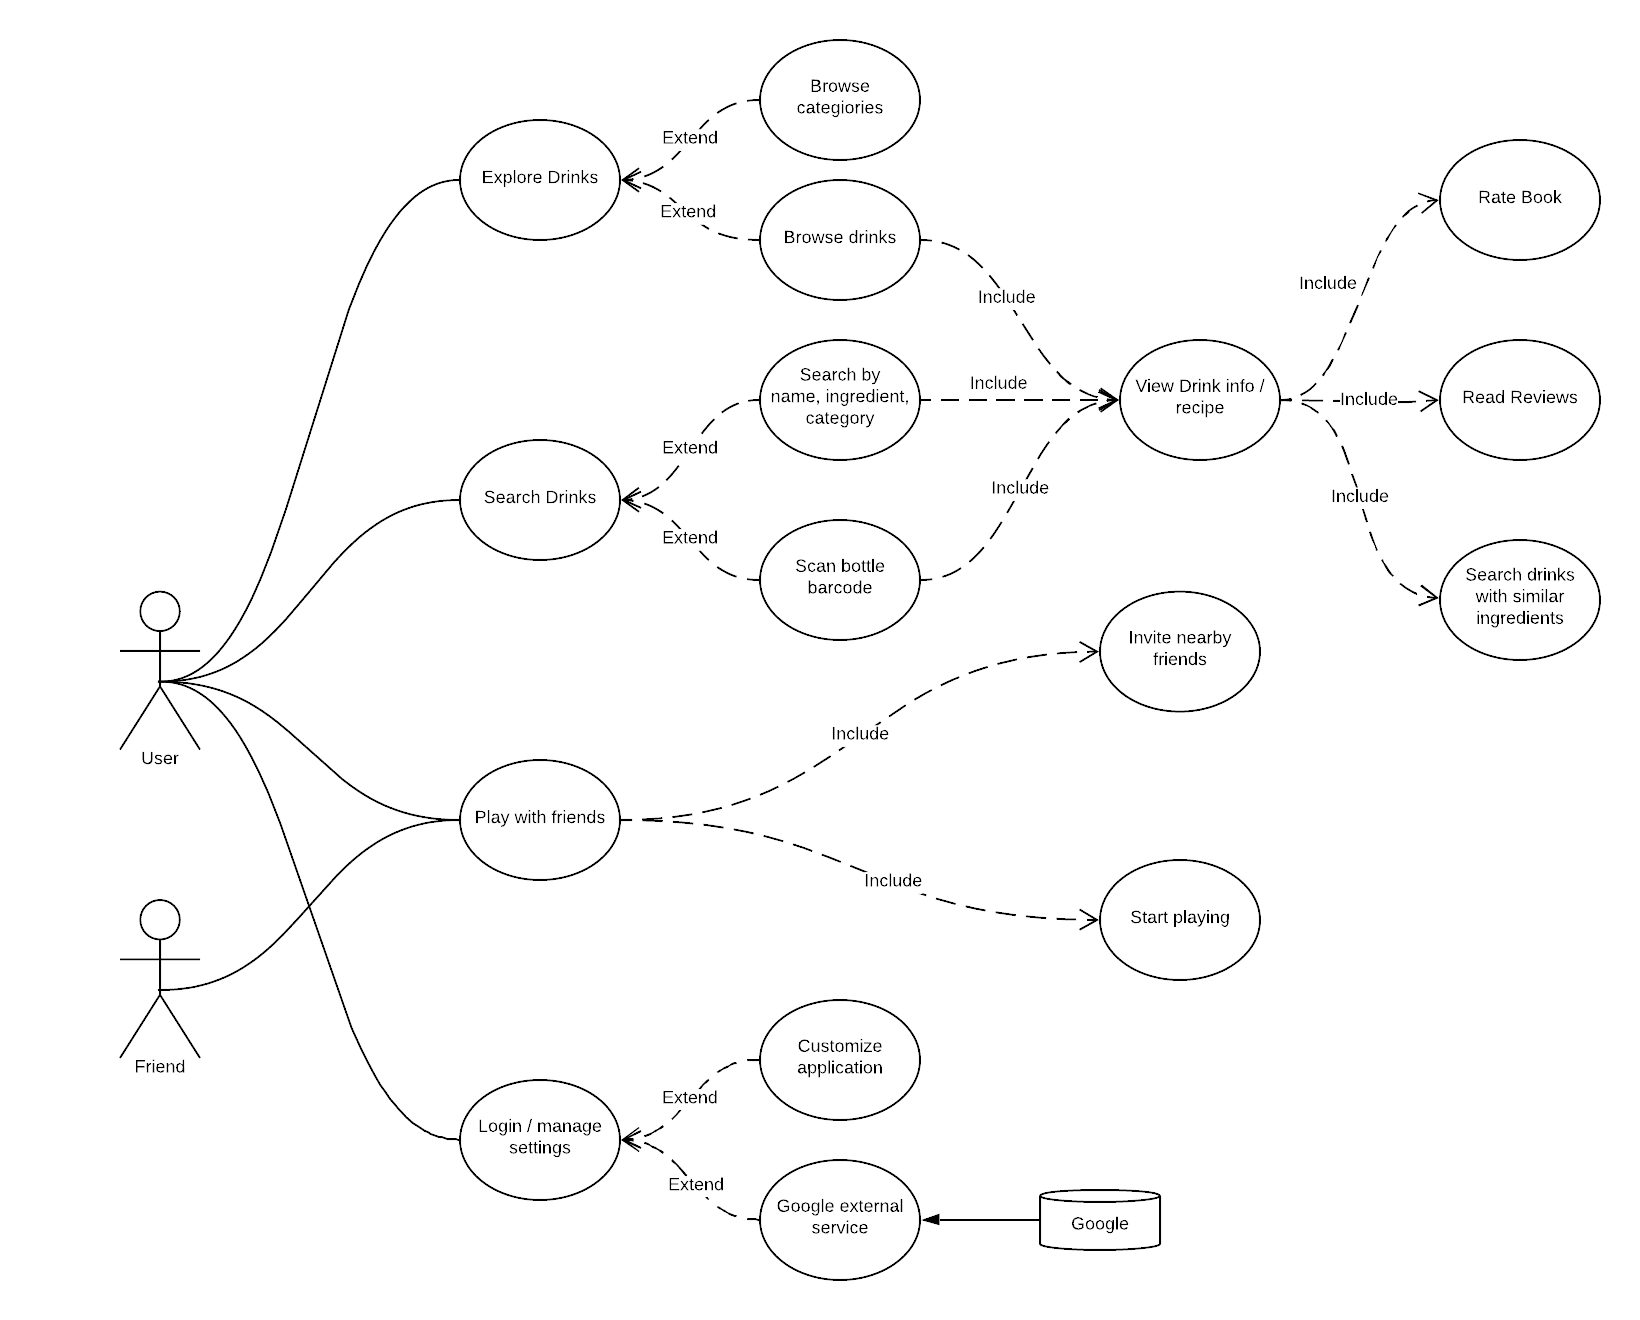
\includegraphics[width=\linewidth]{UseCase.png}
    \caption{eLit - use Case scenario}
    \label{UseCase}
\end{center}
\end{figure}

\begin{enumerate}
    \item \textit{Explore Drinks}: The user can explore our favourite drinks and look for drink categories.
    \item \textit{Search for drinks}: The user can search drinks using any combination of drink name, ingredients, category. There is also the possibility to scan an ingredient bar-code for searching which drinks can be made with that ingredient.
    \item \textit{Drink information}: The user can consult all the information about a drink like the ingredients and all the steps needed to prepare that specific drink, on the iPad version there is also a small description of the drink.
    \item \textit{Set ratings}: The user, once logged in, can write reviews and express ratings for the drinks.
    \item \textit{Play with nearby friends}: The user can invite nearby friends using the Apple’s discovery feature and play with them to a battle quiz game where the questions are randomly generated starting from our drink database.

\end{enumerate}

\subsection{Domain constraints}
In order to have full functionality of the application, few constraint must be satisfied:
\begin{enumerate}
\item The user must have an iPhone or an iPad fully functional, for some optional features like 3D touch preview the version of iPhone must be >= iPhone 6s.
\item The OS version of both iPhone and iPad must be >= iOS 12.0.
\item An access to internet is needed at the first start of the application in order to download and save all the data needed, in general internet connection is not required.
\item For playing games, Bluetooth and WiFi must be enabled, not necessary connected to the internet
\end{enumerate}
\newpage

\section{Architectural Design}

In this section we describe the designed architecture of our application and the parts of which it is composed.

\subsection{Overview}\label{section:overview}

Our system follows a three-tier architecture and can be split up into \textit{Presentation layer}, \textit{Logic layer} and \textit{Data layer}.
Moreover we make use of two external services, namely Google and [?] to achieve all the goals mentioned in the previous section.

\begin{itemize}
\item Presentation layer: This level is composed by the application running on iPhone or iPad. It is going to be what the user will be using and and will overall represent the core tier of our system. The other two tiers will work together to provide information to this layer.
\item Logic layer: This layer will take care of handling all client requests coming from different devices by interpreting them, routing them to the Data layer if necessary, and finally provide meaningful responses.
\item Data layer: This layer is made up by two different databases. One is local to the client application and the other is remotely located on the same machine where the logical layer resides. They work together and the one running on the application can be interpreted as a local storage that provides data to the app immediately without the need to constantly making requests to the server. Moreover the latter one is extremely useful when internet access is not available by providing locally stored data. It is meant to keep a local cache of what's stored on the remote database.
\end{itemize}



%Image

\begin{figure}[H]
\begin{center}
    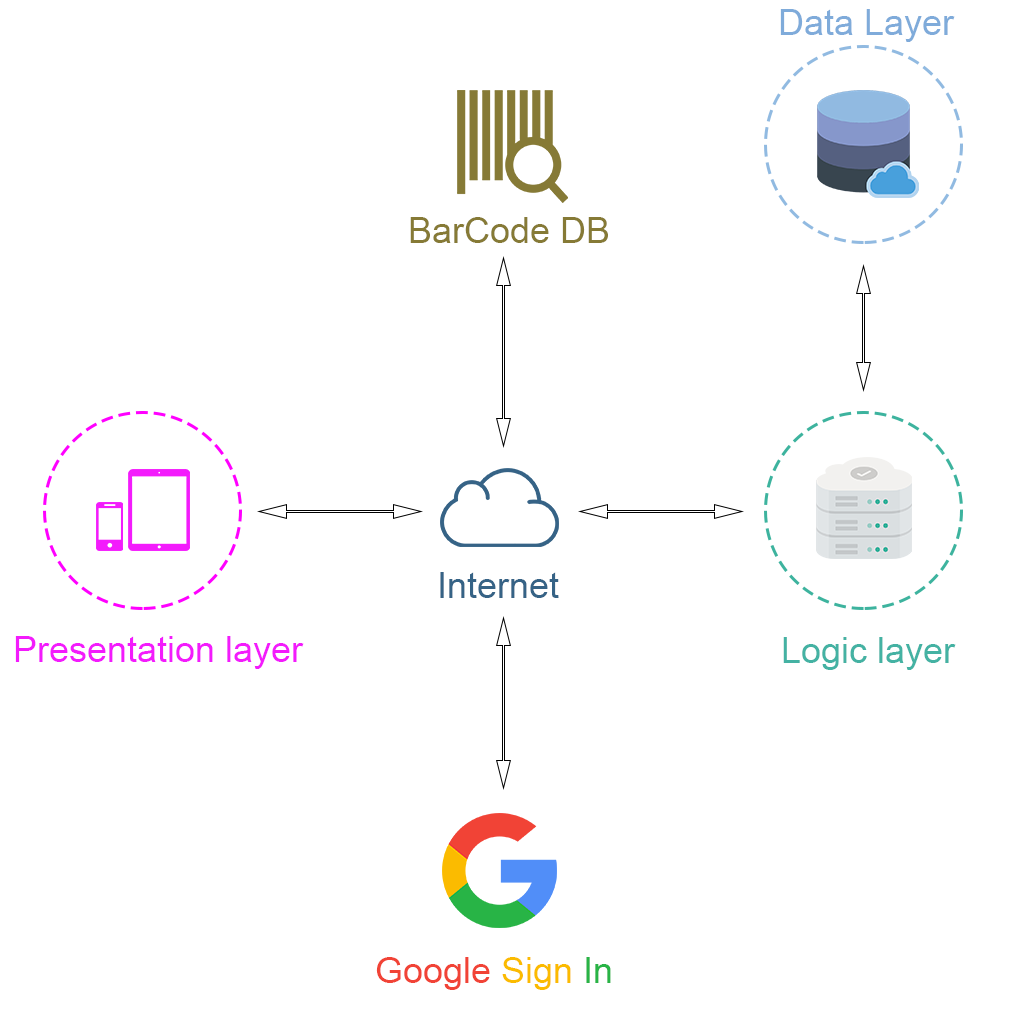
\includegraphics[width=0.8\linewidth]{architecture.png}
    \caption{Three tier architecture design}
    \label{Architecture}
\end{center}
\end{figure}

\ref{Architecture} describes how our system interacts with external services and how it is split up into three tiers. The presentation layer, (i.e. the iPhone/iPad app), uses an internet connection to communicate with the Logic layer. Moreover, it exploits the same communication medium to interact with Google Sign In services and and two BarCode database services, namely \textit{https://world.openfoodfacts.org} and \textit{https://api.upcitemdb.com}, to map codes into meaningful information. 

The logic layer handles requests incoming from the client and responds accordingly, eventually interrogating the Data Layer that resides onto the same machine. 

\subsection{High Level Component View}

% COmp view Image

\begin{figure}[H]
\begin{center}
    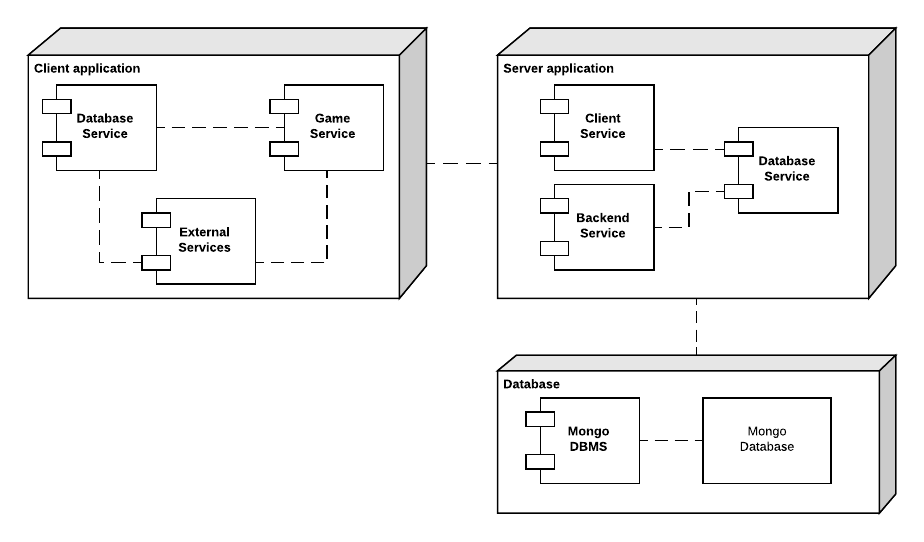
\includegraphics[width=0.8\linewidth]{high_level.png}
    \caption{High level component view}
    \label{High Level}
\end{center}
\end{figure}

\subsubsection{Presentation layer - the app}

In this section we describe from a very high point of view how the client application is structured.

Throughout the development we kept in mind the MVC (Model View Controller) pattern.
We wanted to come up with powerful and clean modules that could have been interconnected and merged together as required. 
The overall result is a combination of services an modules that interact together seamlessly.

Together they take care of storing and retrieving data when needed, making request and fetching responses to the server and interact with other devices. Their whole implementation is asynchronous so that the applications always remain responsive.

We herby split these services into the following ones, even though we are describing them from a very high level point of view.

\begin{itemize}
\item  First is the \textbf{Database Manager Service}. All the information that is displayed to the user, i.e. cocktails, recipes, ingredients and so on, are stored locally on a databases implemented using Apple's CoreData framework. This databases is filled the first time the app launches and is kept up to date by the Database Manager Service, which ensures that all data present onto the remote database is mirrored into the local one. This way, should the internet connection ever be not available, the app will always display something to the user without crashing or reporting any error. On every startup it inquires the remote servers for updates of regarding all the assests and reacts accordingly to the response. Moreover it stores user information and tracks preferences changes.
\item Next up is the \textbf{Game Manager Service}. Giving the user the possibility to play with other people required us to design a specific service that exploits Apple's \textit{MultipeerConnectivity Framework} to enable Peer2Peer connectivity between multiple devices throughout \textbf{WiFi} or \textbf{Bluetooth}. The framework uses infrastructure WiFi networks, peer-to-peer WiFi and Bluetooth personal area networks for the underlying transport. Our service builds on top of the latter framework one and enables the connection between two devices, handles invites, connection drops, and most importantly takes care of the whole game logic, granting the user a great experience.
\item Finally we exploit two external services: \textbf{Google SignIn} and \textbf{2 BarCode databases}. Google's services are used to authenticate the user and get his profile data. Moreover, to fulfill the goal of letting the user scan any BarCode, we developed a module that interfaces itself with these external services. Upon requests the latter ones provide a meaningful response that is then parsed and used to display results to the user. These services will be discussed more in-depth later or.
\end{itemize}

\subsubsection{Logic layer - the server}

The server application is made up by three core services, again from a high level point of view, and each one tackle a different task.

\begin{itemize}
\item The requests that come into the application server from the various clients (i.e. iPhones and iPads) are handled by the \textbf{Client Service}. It is build on top of a standard HTTP Server and is queried throughout a RESTful interface. 

On every launch the app reaches out at the server to ask for updates and this service is responsible for checking whether or not the client's local database is out of date. If so it serializes the updated information and sends it over the network exploiting the REST API. This module interacts directly with the \textbf{Database Service} and interrogates it whenever it needs to.
\item The \textbf{Database Service} is responsible for querying Data Layer and parse the results. It can be seen as an abstraction over the Database in order to have a transparent way of fetching information.
\item Finally, the \textbf{Back-end Service}, again built on top of the same HTTP Server mentioned above, handles all the request that come from the Web GUI designed for ELIT administrators only. It is meant as a Graphical User Interface to manage all the cocktails, recipes, ingredients and all the other assets present in the database.  

Communicates directly with the Database Service which updates the Data Layer accordingly.
\end{itemize}


\subsection{Data Layer - the database}





The data layer is composed by two different databases, one is located server side and is used to fetch all the data from the application when it is opened for the first time, the second one is located inside the application in order to have a more responsive application that can works even without internet connection.

\subsubsection{Application database}
The application database is a relational database powered by Apple's framework called Core Data and is used to store all the information about drinks and the user profile. Every entity inside our model has a parent abstract entity called CoreDataObject that we have used to better interact with the object inside our database.

The User table keeps track of all the information about the user when he logs in for the first time and is updated every time the logged user changes. This is useful in order to keep the information that will be used for writing reviews and for playing games.


All entities that  are related with the drinks have a parent entity called Drink Object which keeps a unique identifier and a fingerprint that are given from the remote database and are used for updating the drinks. A Drink is composed by a Category and a Recipe, the Recipe is an ordered list of RecipeSteps which are composed by a collection of DrinkComponents each one with his own Ingredient.

All the entities that have an image (in our case the drinks and the ingredients) have as parent entity DrinkObjectWithImage that keeps the image data attribute that is fetched from an url the first time is requested by someone and then saved into the persistent model.\par
As mentioned before, the entire schema is fetched one time at the first application start and then is updated (if an internet connection is present) every time the application have been opened.

\begin{figure}[H]
\begin{center}
    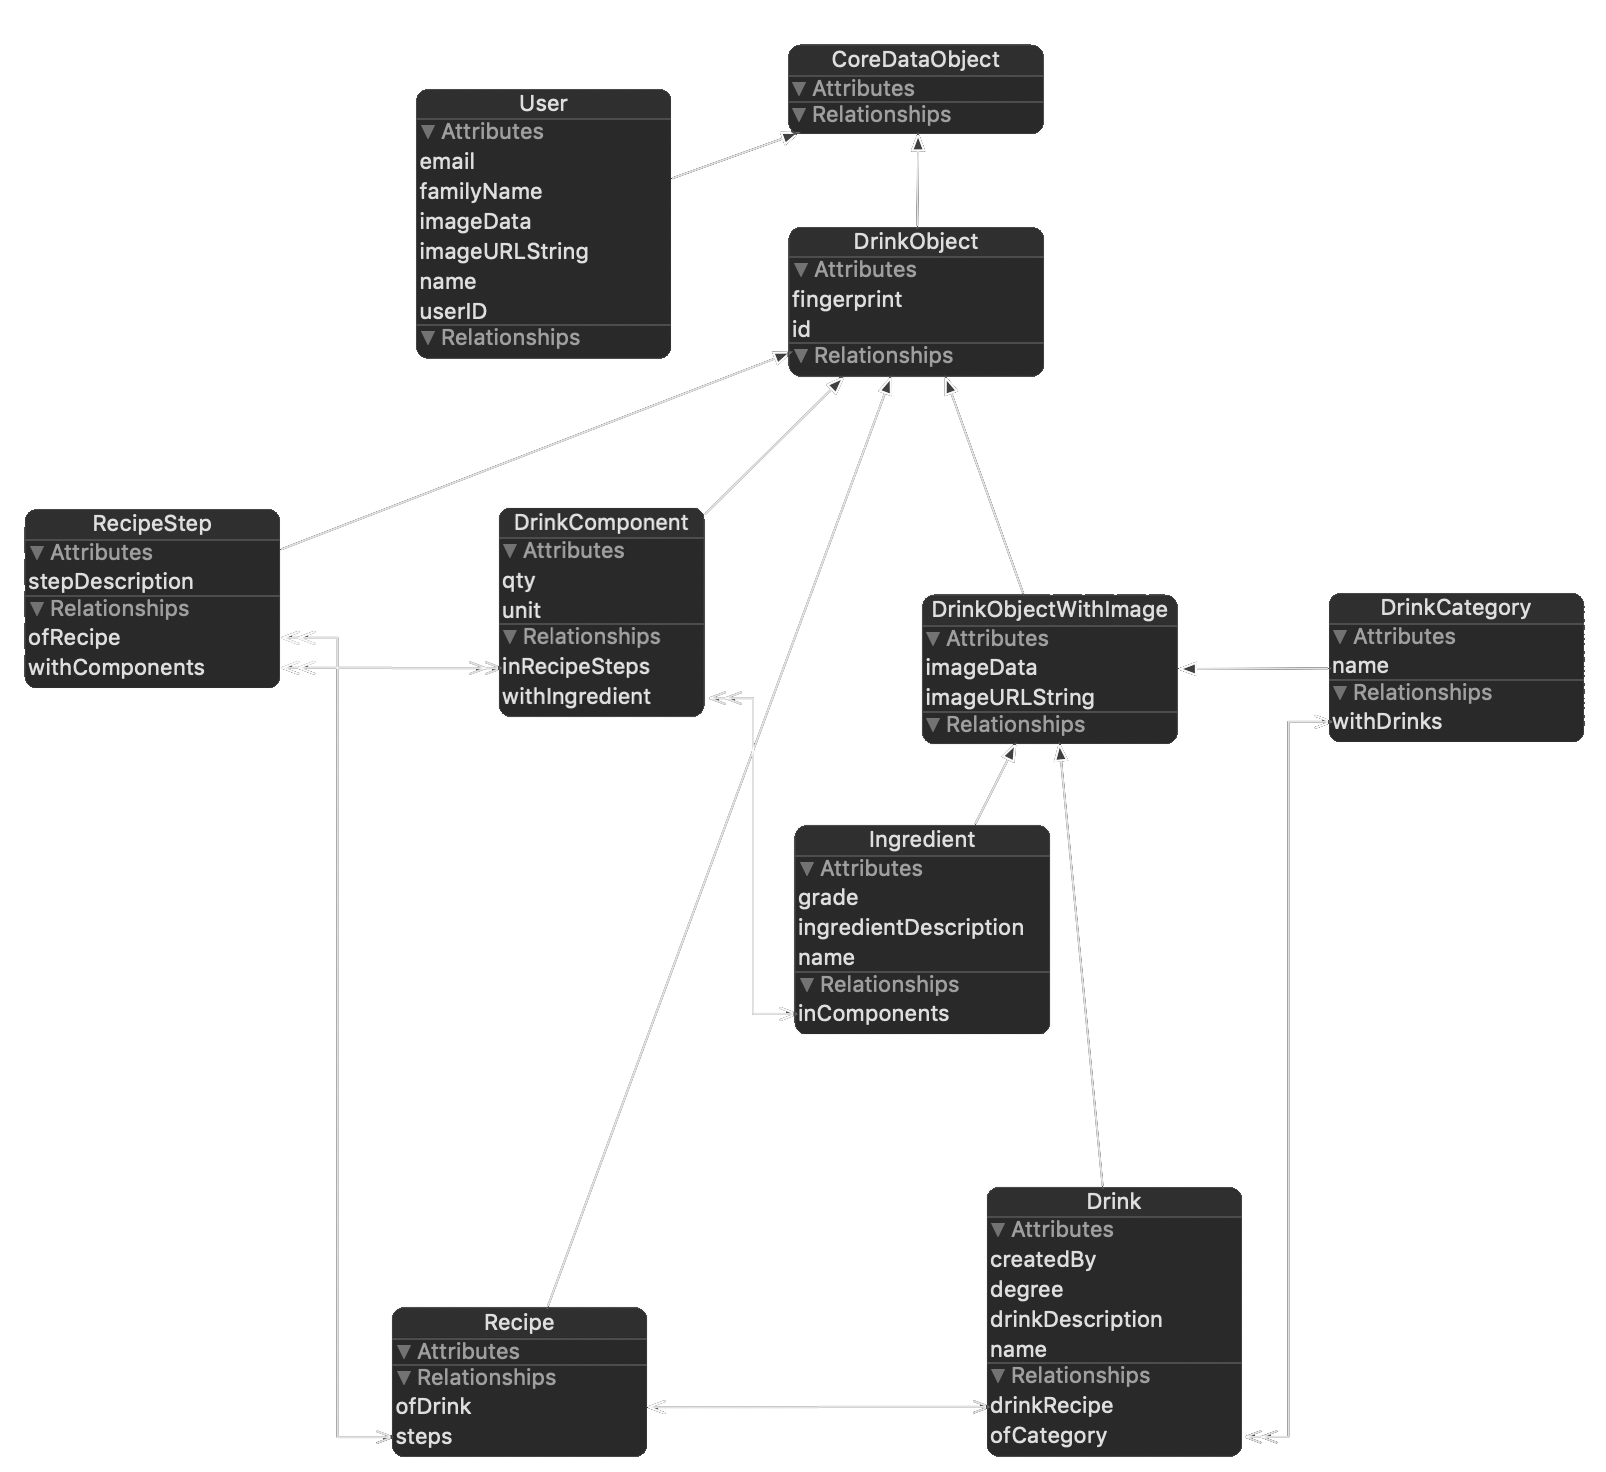
\includegraphics[width=\linewidth]{entities.png}
    \caption{Application database entities}
    \label{Database entities}
\end{center}
\end{figure}

\subsubsection{Server Database}
The server database is No-SQL MongoDB database hosted into our server and accessed by a REST API. In this schema we store all the information about drinks with the same structure of the application database. We also have the information about our registered users and about the reviews they have written. The User registration is provided by Google authentication and once an user have been logged in we sand the information to our server.

\begin{figure}[H]
\begin{center}
    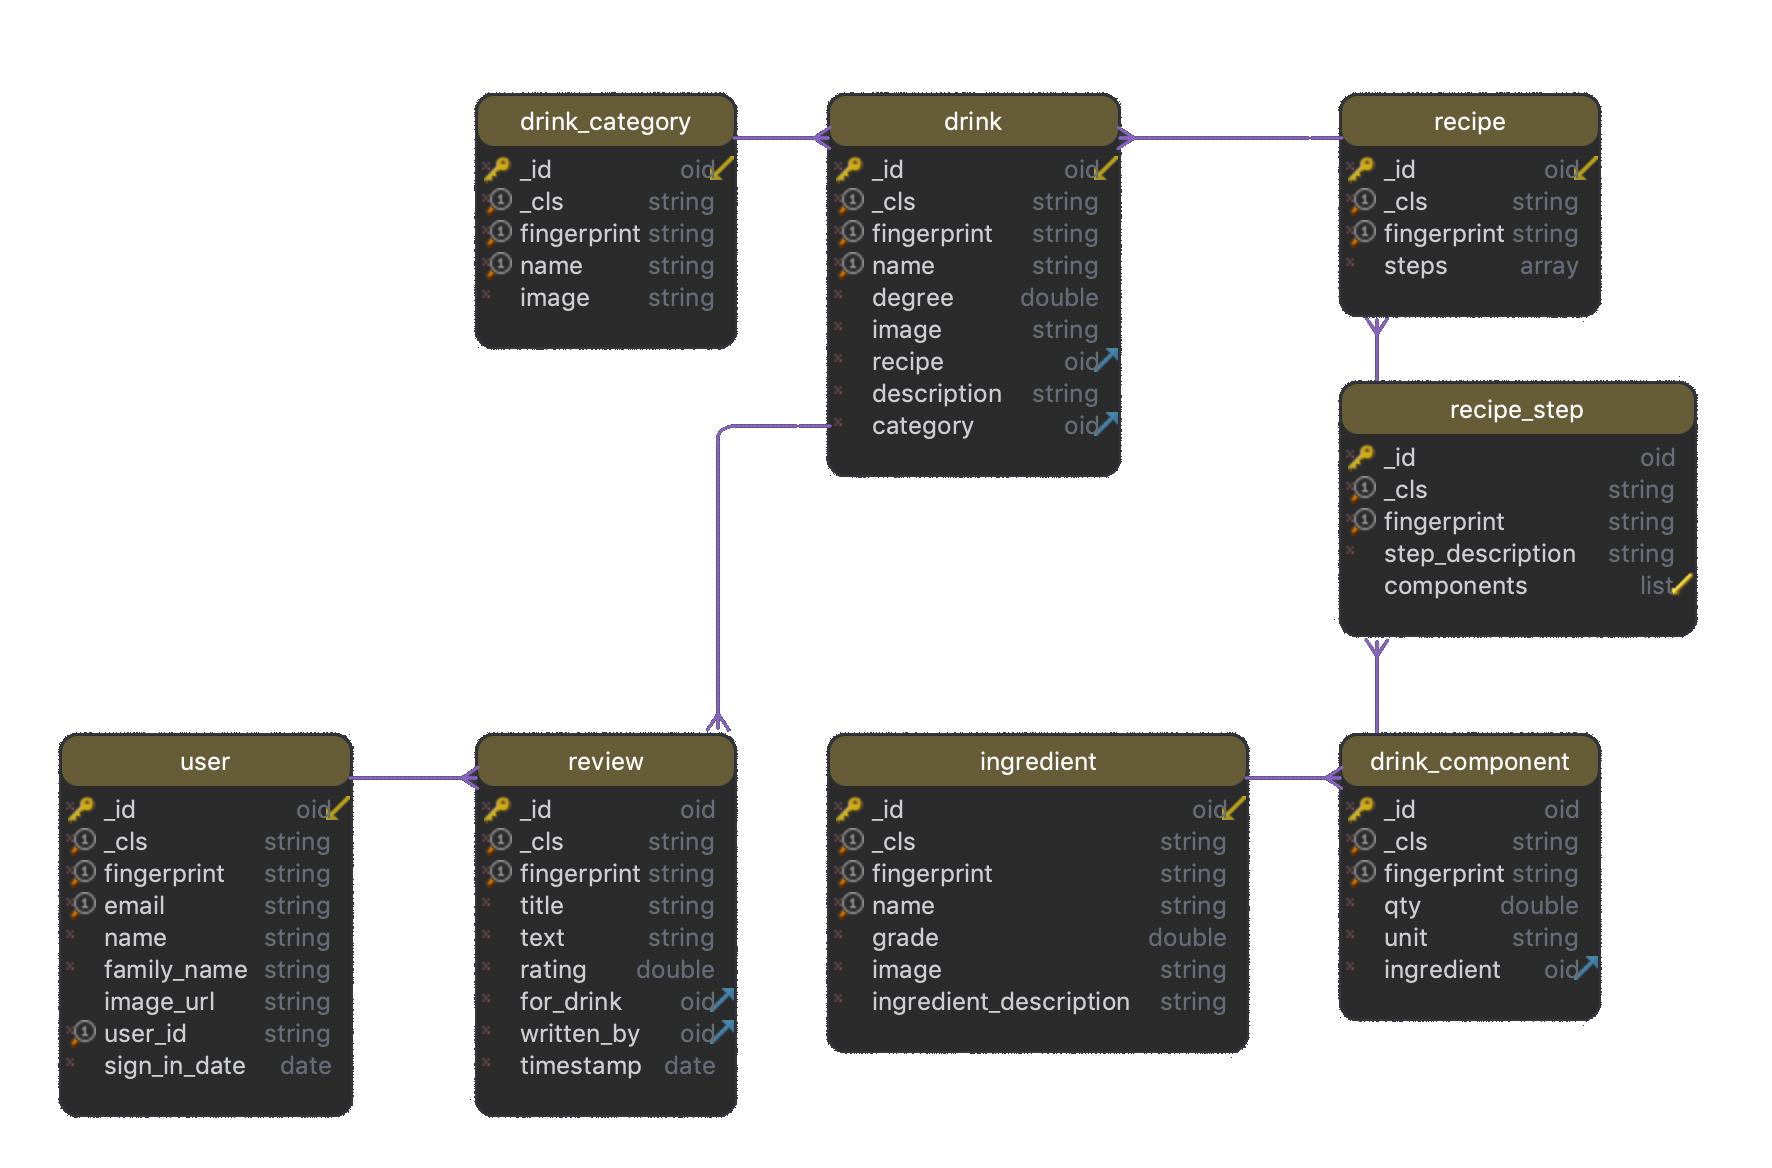
\includegraphics[width=\linewidth]{ServerDB.png}
    \caption{Server database entities}
    \label{ServerDB}
\end{center}
\end{figure}

\subsubsection{External services}\label{section:external services}

\section{User interface design and functionality}
When it comes to mobile development designing a good-looking and responsive user interface is as much important as designing the rest of the architecture. 

With this in mind we started developing a modular and flexible set of UI components that could be mixed together and swapped at our own needs. The overall result is a design which is made up of \textit{blurs and vibrant views} that makes the app look beautiful in all of its sections.

\subsection{Multi-device support and size classes}

In order to fulfill the requirements that a modern application usually exposes, we decided to develop an app that would look great both on iPhones and iPads by working with \textbf{Apple's Size Classes} that allowd us to fine tune components alignments and much more. However we even had to re-design and re-engineer some sections, such as the Home and the Cocktail detail, because it simply wasn't enough tuning these parameters and content needed to be displaced in a totally different manner. 


\subsection{Design strategies and features}

Inspired by the design
 that Apple uses for most of its own apps, such as the App Store, we opted to hide navigation bars and use the so called \textbf{Large Titles} to identify sections of the app. This feature has been available since iOS 11 and integrates greatly with our design strategy, whose objective was to make fage of the available screen space.

Furthermore it is worth noticing that our design is dynamic, in that it depends on the rendered assets and is capable of reacting accordingly. For instance, in the home section, depending on the current selected category on the top carousel, the background will blur to shades that recall the category image every time the user swipes through them. This ensures the user has a dynamic experience and even some feedback out of the actions he is performing while using the application (See figure \ref{Titles}).


Moreover, the app has two themes: \textbf{Standard theme} and \textbf{Dark theme}. We will present the former while going through the various sections and the latter will be addressed later on.

\begin{figure}[!ht]%
    \centering
    \subfloat{{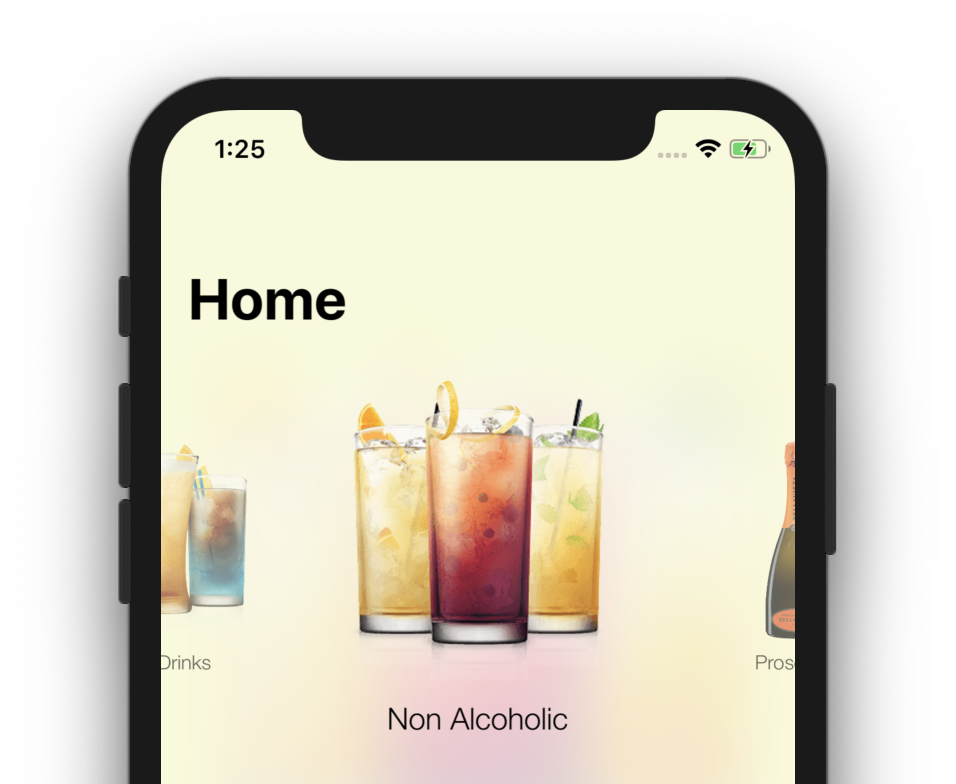
\includegraphics[width=7cm]{UI/UI-Title-L.png}}}%
    \qquad
    \subfloat{{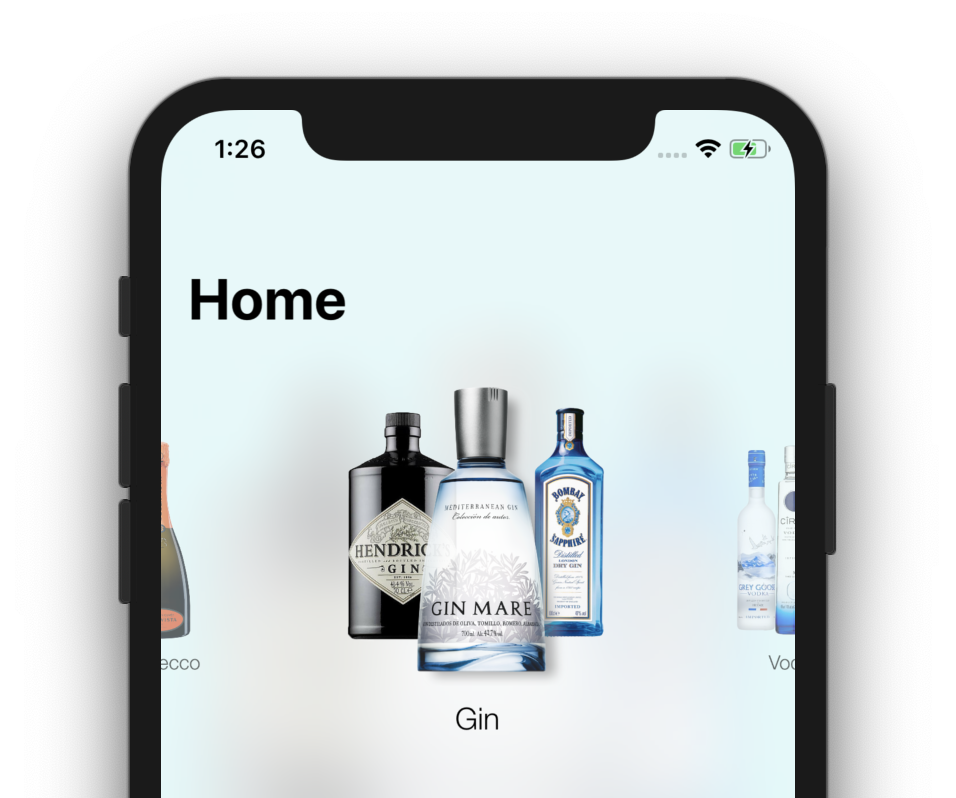
\includegraphics[width=7cm]{UI/UI-Title-R.png} }}%
    \caption{Large titles and blurred, vibrant and responsive design}%
    \label{Titles}%
\end{figure}

\begin{figure}[!ht]%
    \centering
    \subfloat{{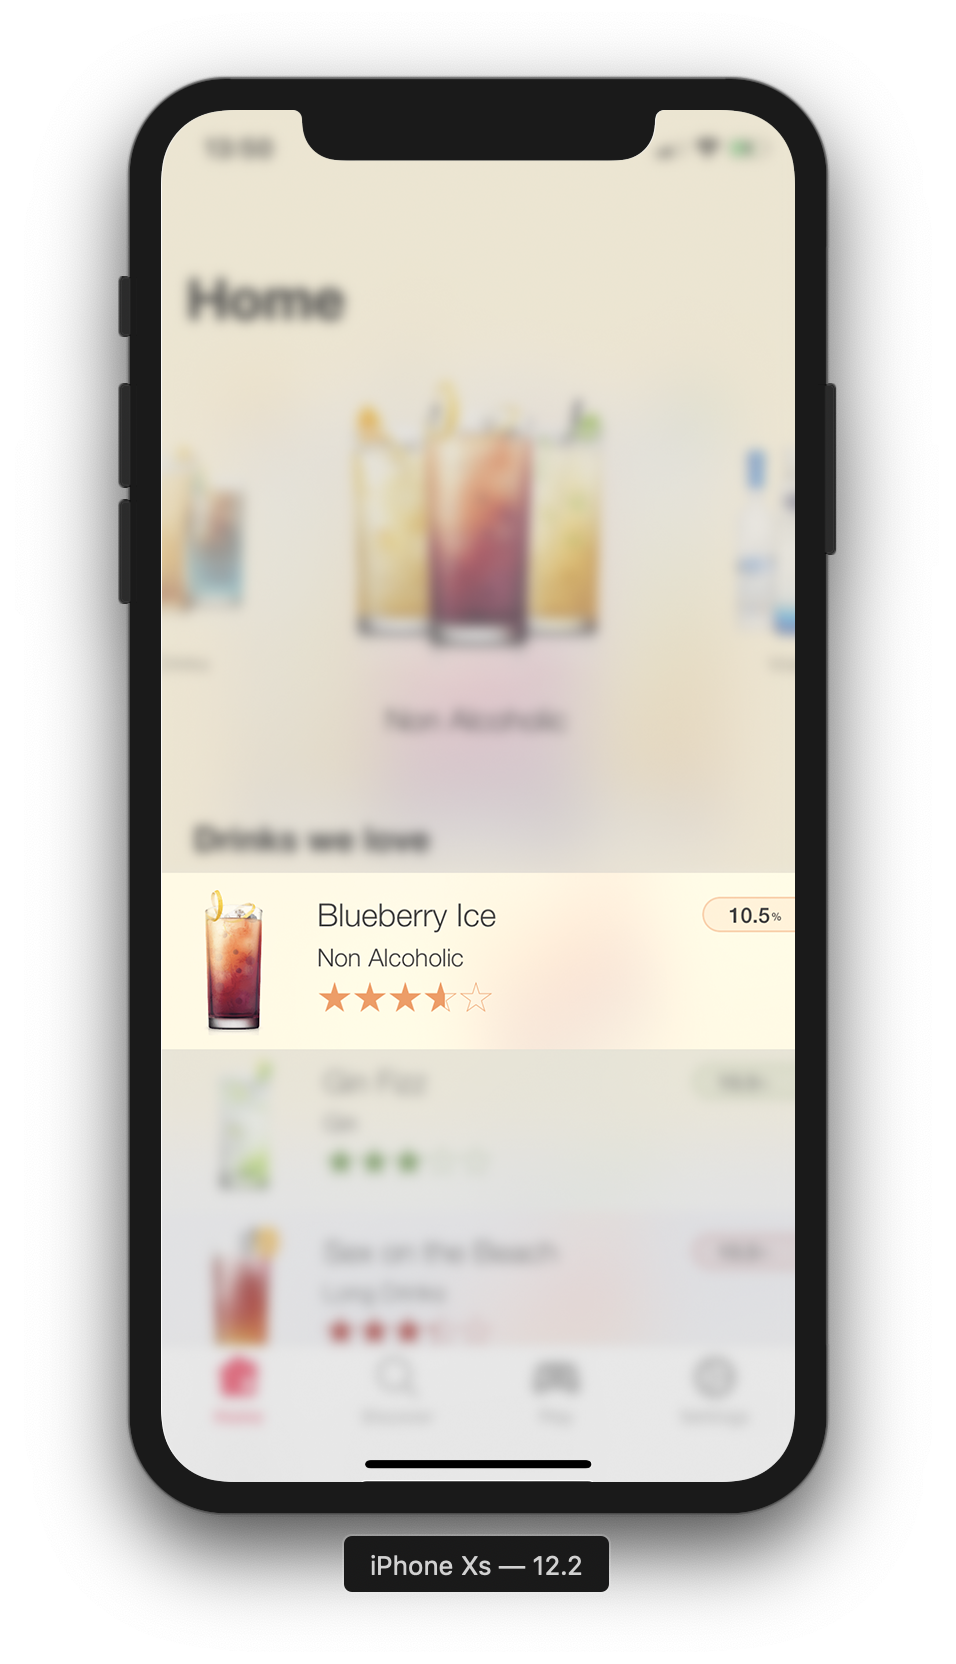
\includegraphics[width=7cm]{UI/UI-3D-opening.png}}}%
    \qquad
    \subfloat{{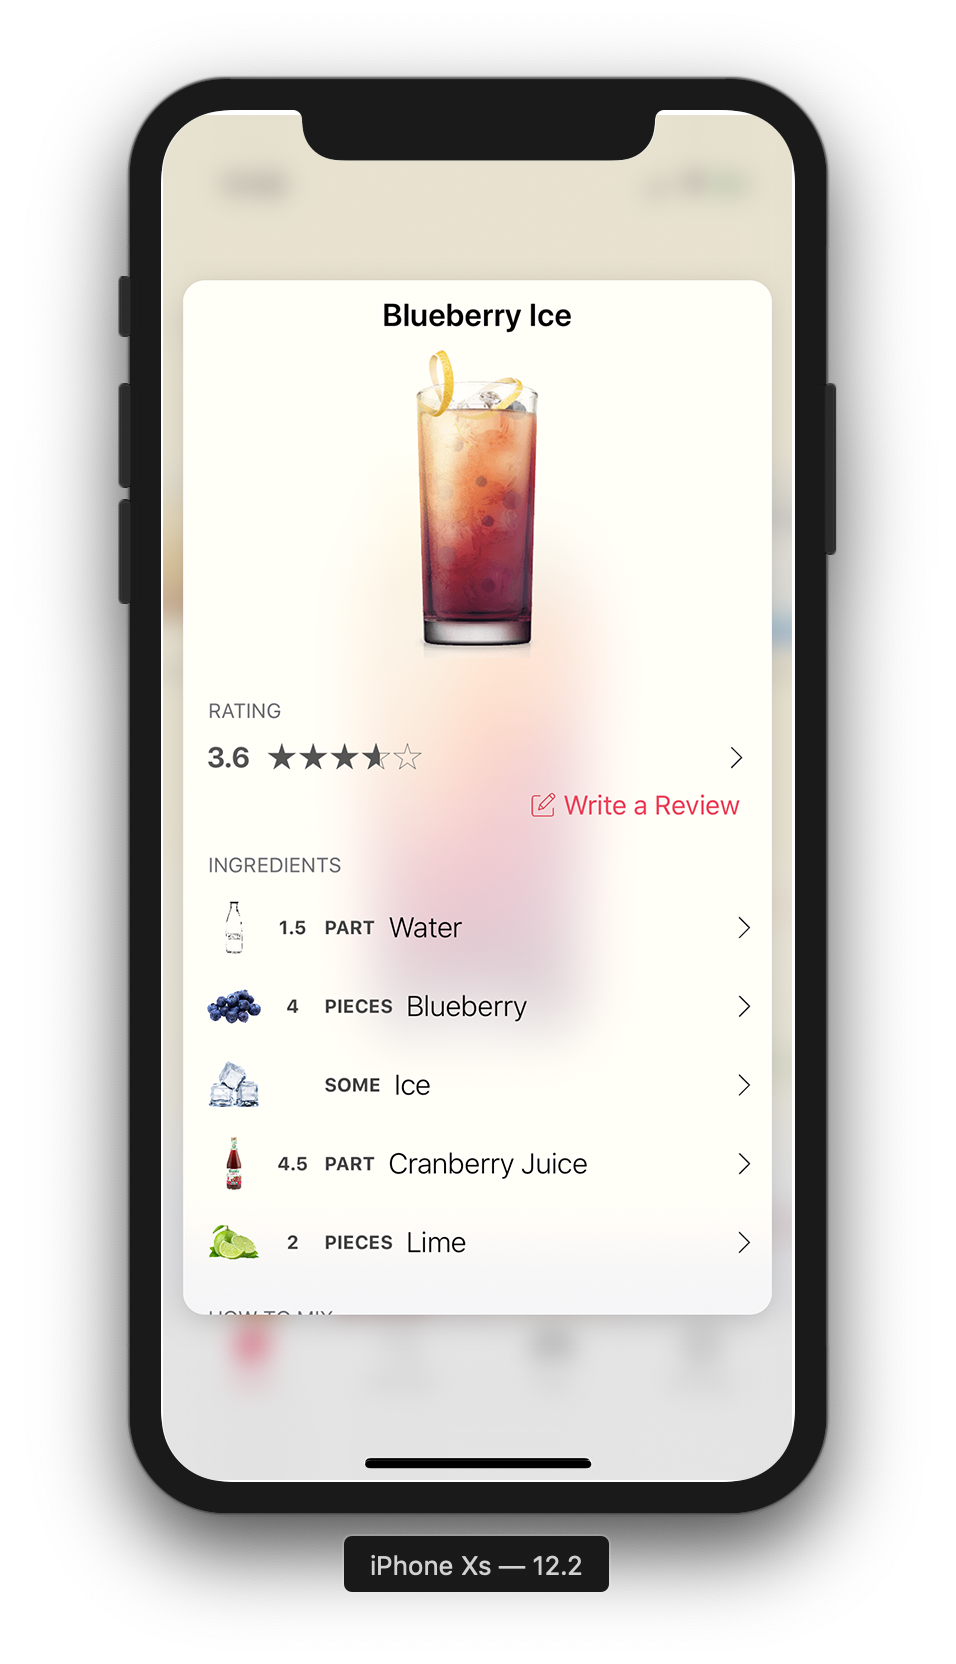
\includegraphics[width=7cm]{UI/UI-3D-open.png} }}%
    \caption{3D Touch support}%
    \label{3dtouch}%
\end{figure}

Our application integrates \textbf{3D Touch Support} and it has been implemented in the home section as drink preview feature in the cocktail list. In figure \ref{3dtouch} we provide an example of this feature.

Finally, we decided to lock device orientation in portrait mode by disabling landscape support.

\subsection{Application sections}

The application is divided into four main sections:

\begin{enumerate}
\item \textbf{Home} : this section is responsible for providing and overview onto categories and drinks to the user. 
\item \textbf{Discover} : this section allows the user to search through categories, drinks and ingredients as well as scanning bar-codes.
\item \textbf{Play} : This section handles everything related to gaming, such as player discovery, invitations and in-game actions.
\item \textbf{Settings} : This section gives the user the possibility to log-in and log-out, toggle preference switches and changing app theme.
\end{enumerate}

\subsubsection{Home section}

This section is responsible for presenting the user drink categories and cocktails themselves. It is one of the most important sections of the app and is the one shown after launch. In order to provide the best experience possible to our users we had to re-engineer the way in which content was being displayed according to the device used. However both iPhones and iPads offer the same exact functionalities crafted with different design.


\begin{figure}[!ht]%
    \centering
    \subfloat{{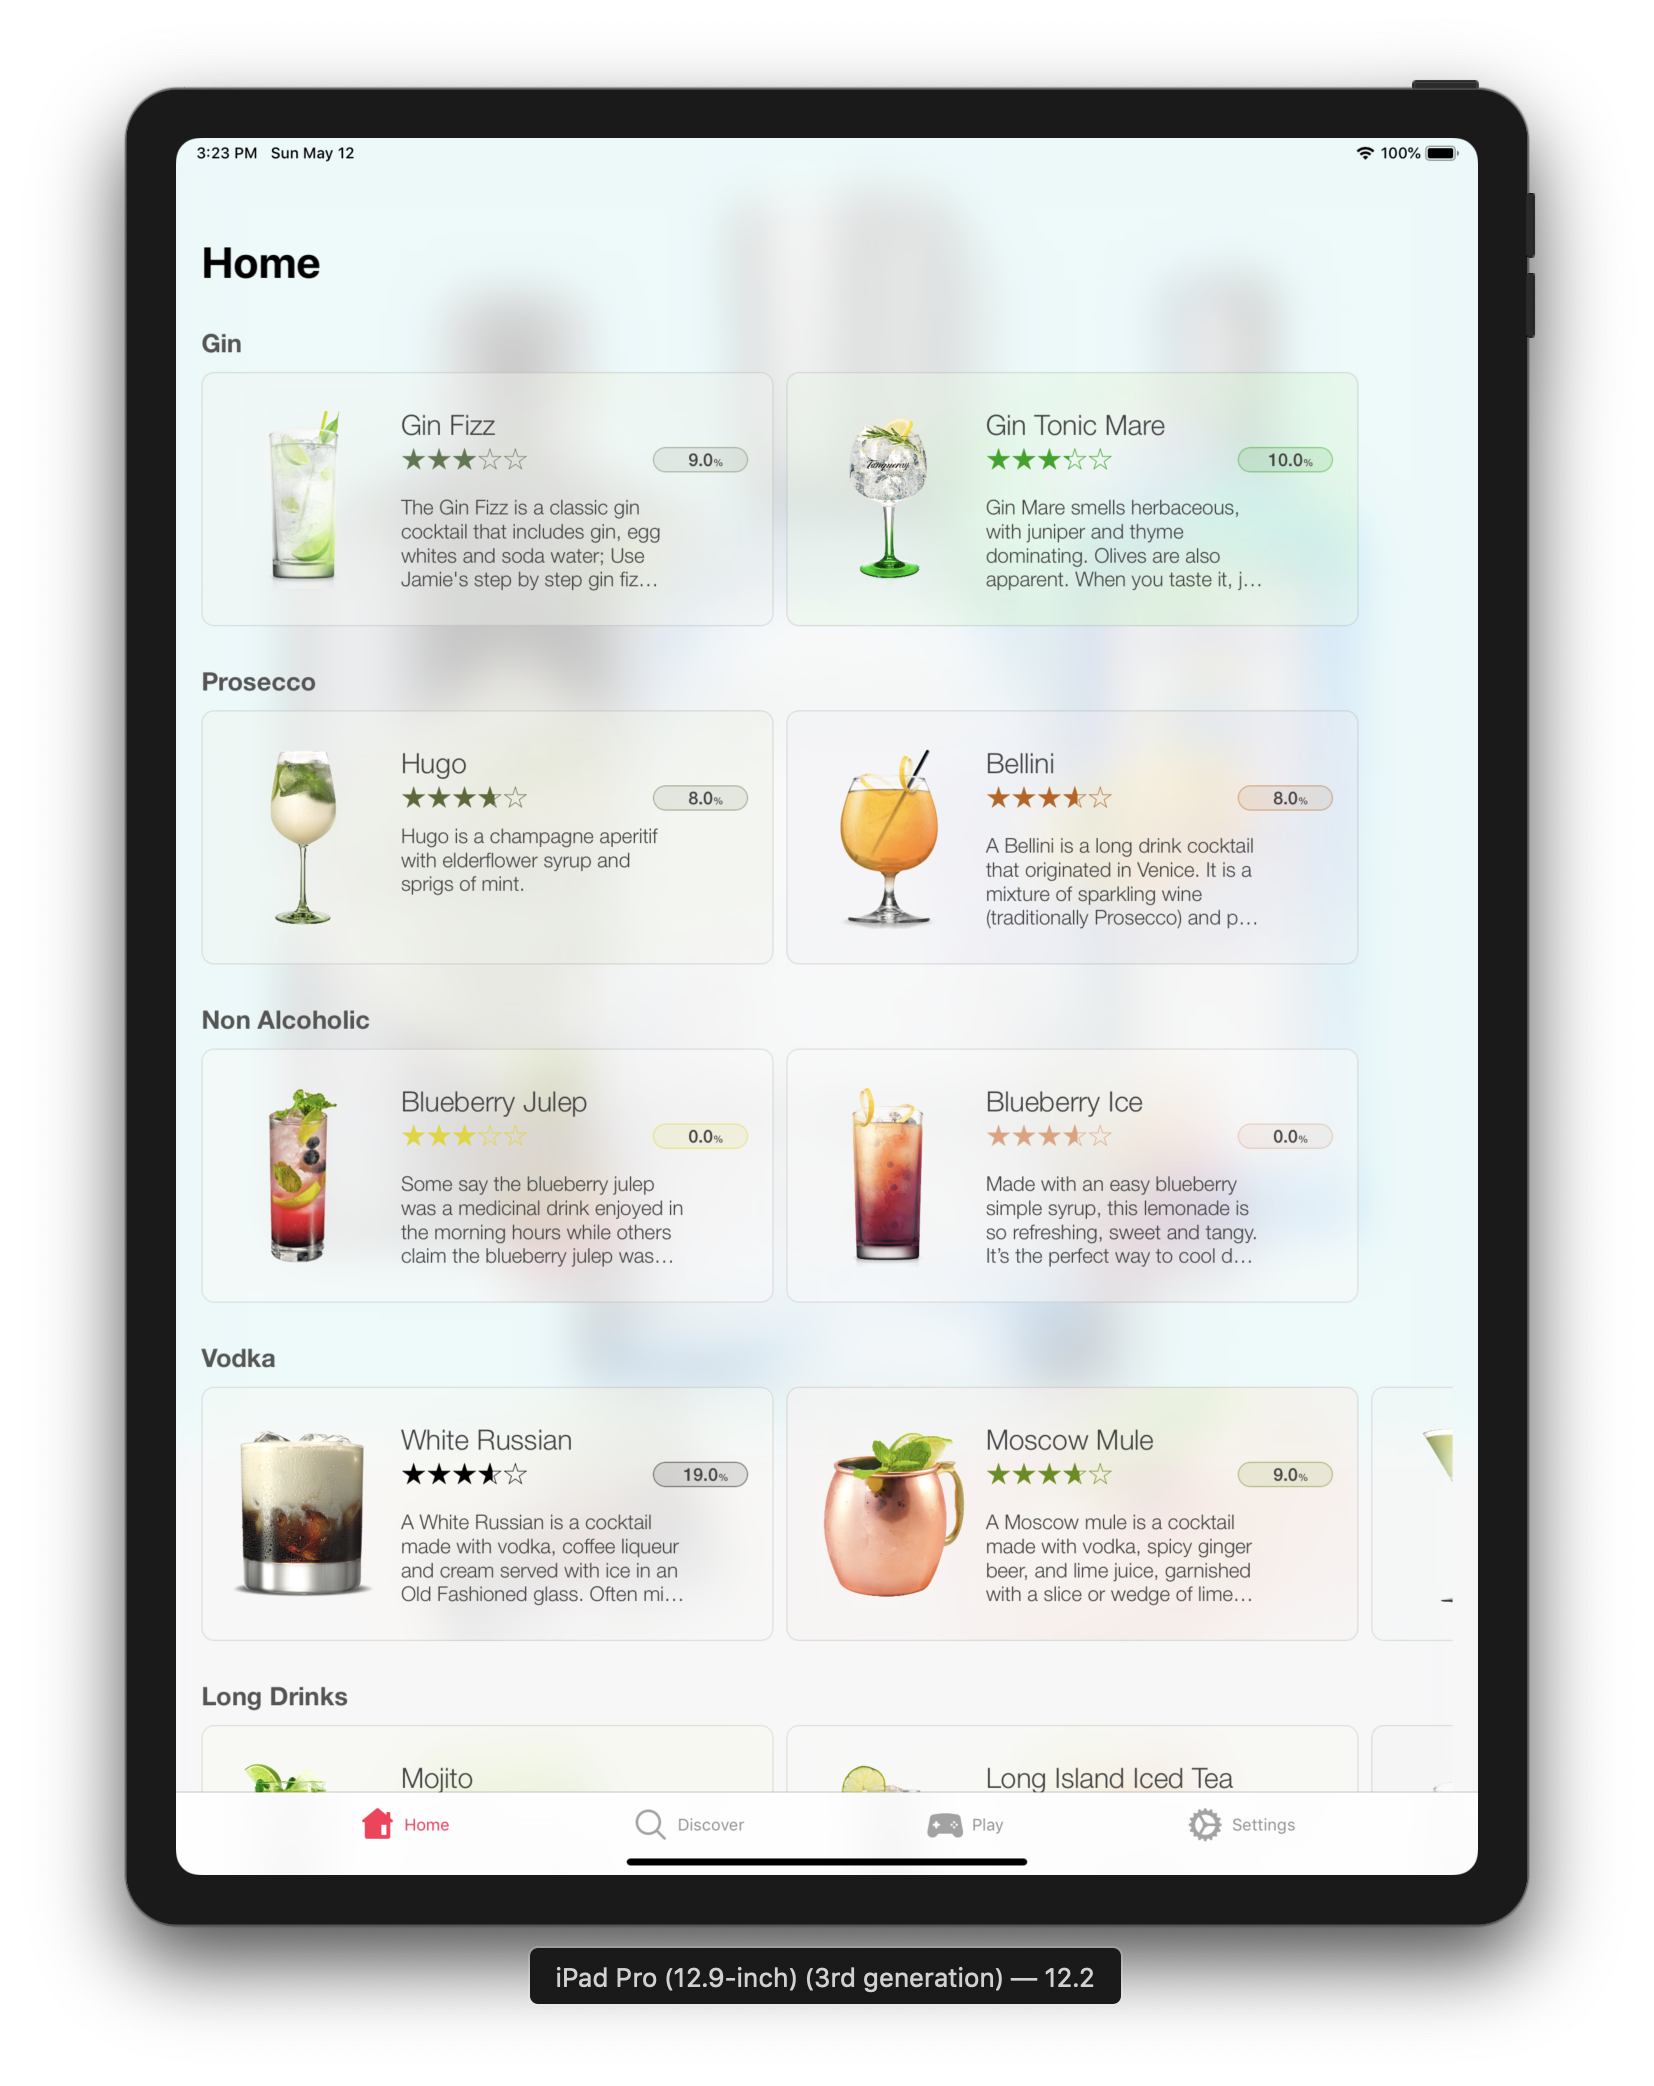
\includegraphics[width=8.1cm]{UI/UI-Home-ipad.png}}}%
    \qquad
    \subfloat{{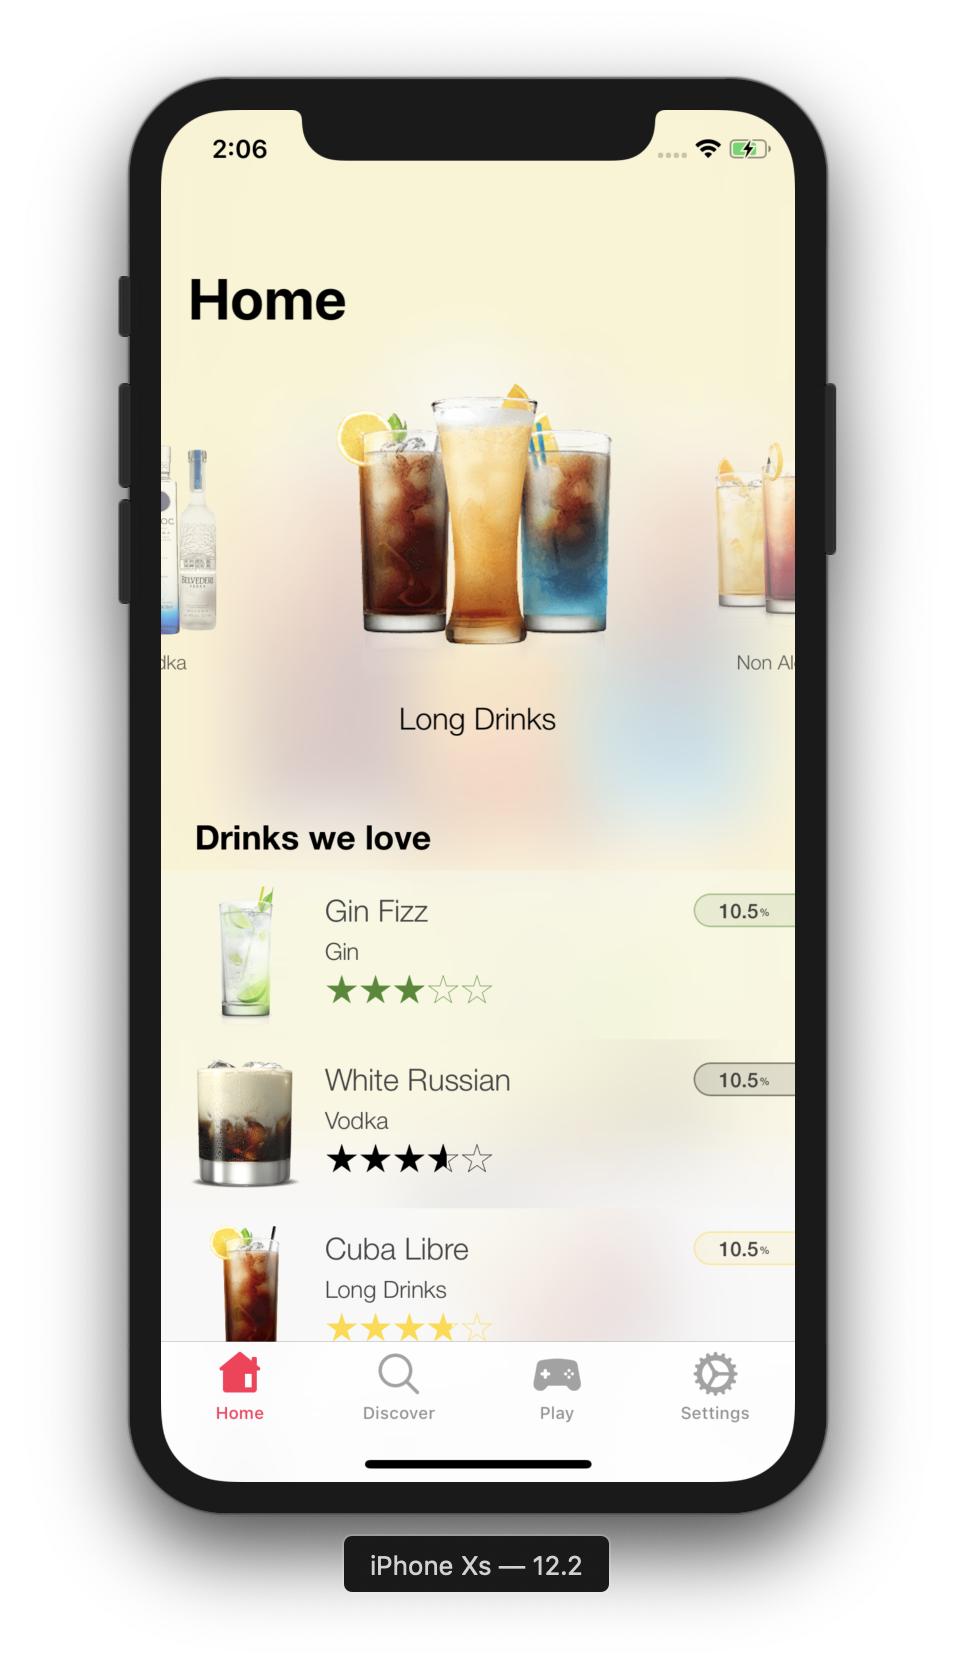
\includegraphics[width=5.9cm]{UI/UI-Home-iphone.png} }}%
    \caption{Home section overview on iPad and iPhone}%
    \label{home section}%
\end{figure}

\begin{itemize}
\item  \textbf{iPhone} : on iPhones we find two core components:

The first one is a carousel that allows the user to browse between categories. Upon touch, the user is presented with a list of drinks that belong to the chosen category. Swiping through the categories will change the background blur and colors of this view.

The second component is a vibrant table view that present a list of available cocktails. For each one we report its name, category, community rating and alcoholic degree.
\item \textbf{iPad} : the content for iPads have been adapted to show information in a much more clean way that takes advantage of the screen. More specifically the carousel has been removed and the user is presented with a table where each row represent a different category of cocktails with an embedded collection view.
The latter one allows for horizontal scrolling of all the drinks that belong to that category.
\end{itemize}

\subsubsection{Discovery section}\label{section:discover}

This section allows the user to search for drinks, categories and ingredients. While typing the user is presented with live results related to what he is searching. When nothing is present in the search bar, there is a huge button in the middle of the view that allows the user to scan bar-codes.

\begin{figure}[!ht]%
    \centering
    \subfloat{{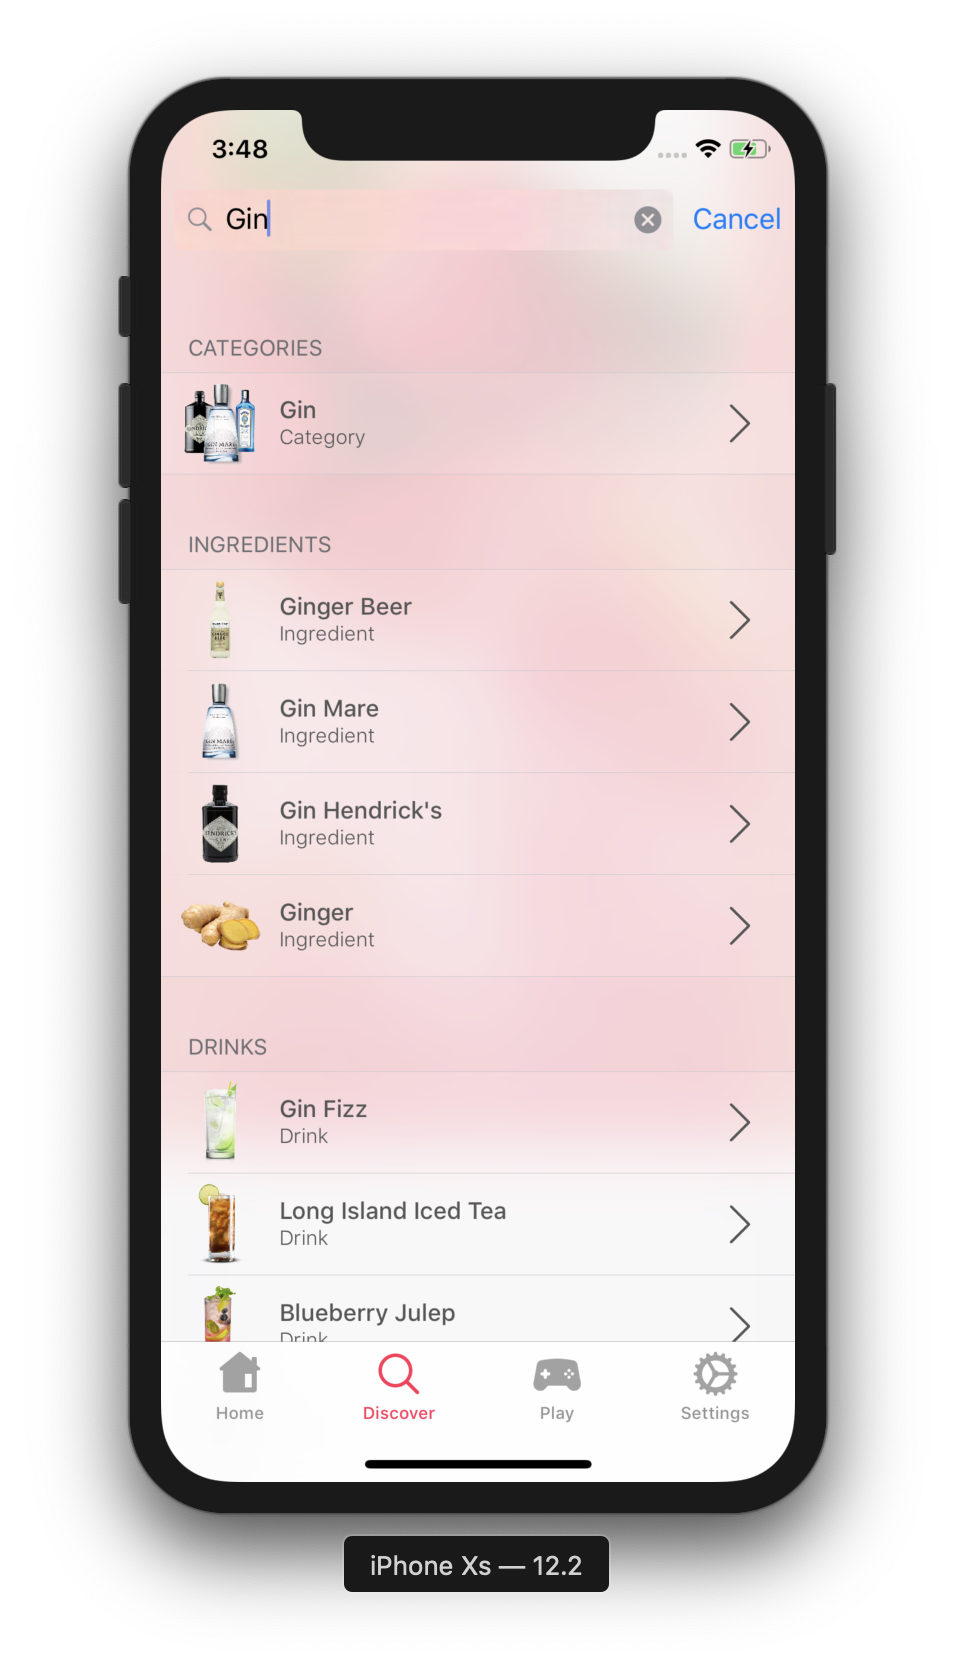
\includegraphics[width=7cm]{UI/UI-Discover.png}}}%
    \qquad
    \subfloat{{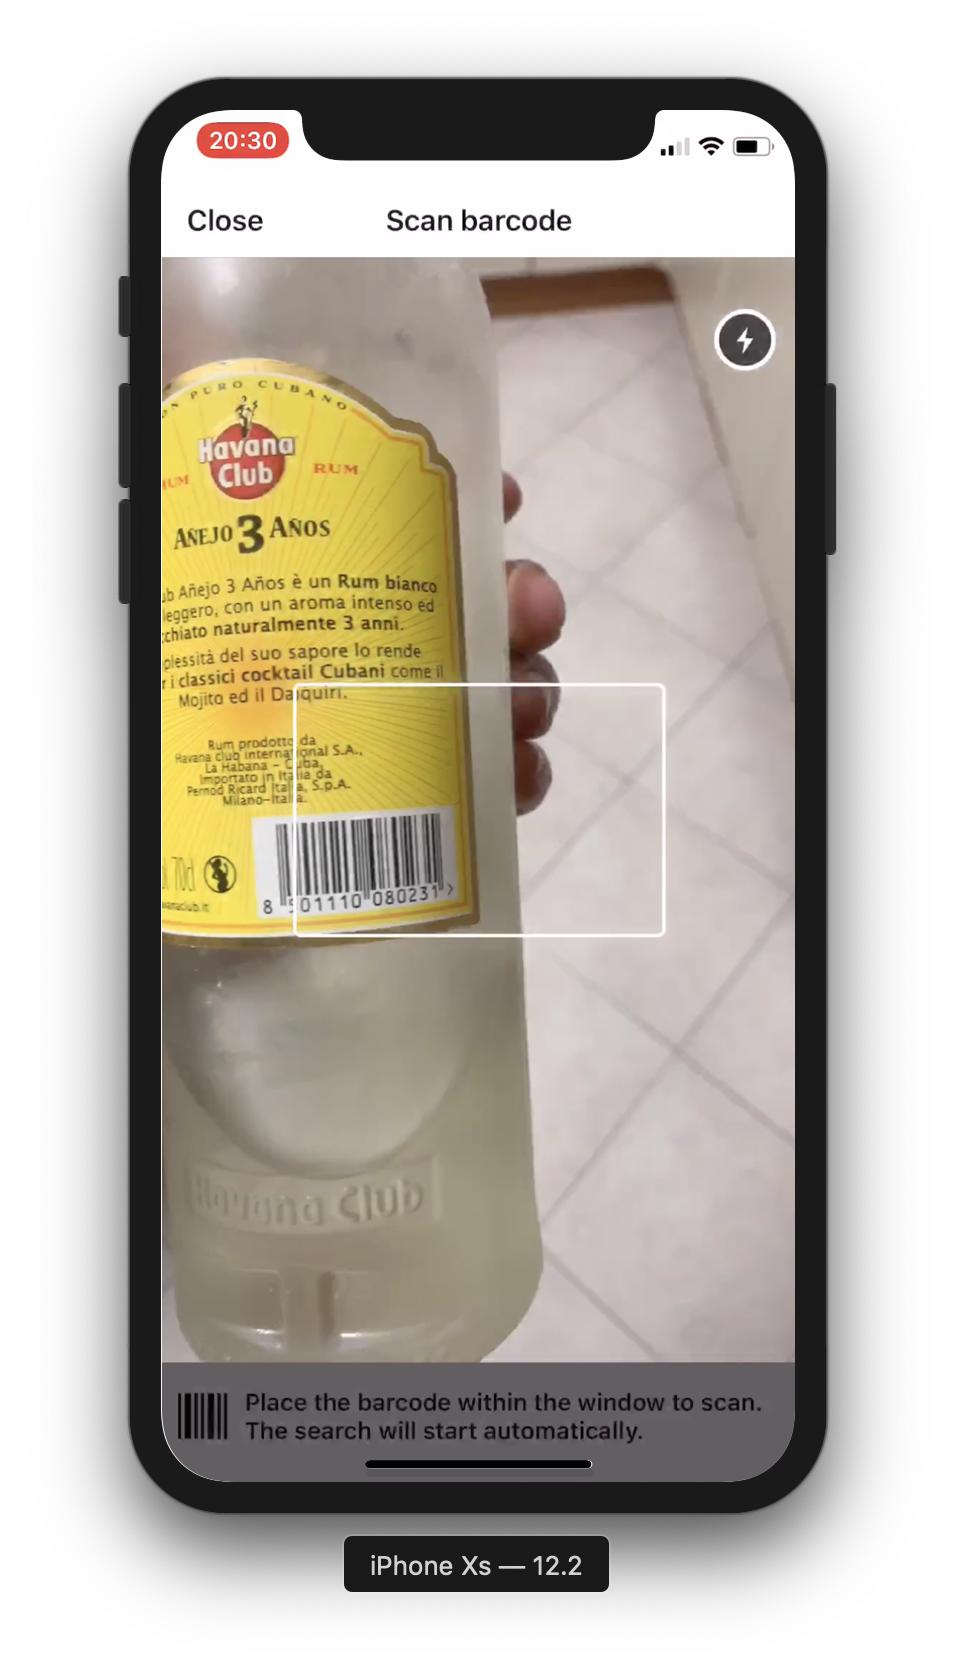
\includegraphics[width=7cm]{UI/UI-barcode.png} }}%
    \caption{Discovery section with results for the query "gin" and a screenshot taken from the bar-code scanner}%
    \label{discovery section}%
\end{figure}


\subsubsection{Play section}

This section is responsible for allowing the user to play with nearby friends.
When opened, the application starts advertising itself using infrastructure WiFi network, peer-to-peer WiFi and Bluetooth personal area network. At the same time it starts looking for other players in the surrounding area. 

When a device is found, he is displayed in a table with a button that enables invitation. Upon touch, the remote peer is asked to either accept or decline the invitation within a time frame that lasts for 30 seconds. If the user doesn't perform any action the invite is automatically declined.

If the remote peer accepts the invitation, the game starts and both players are presented with a set of five questions. Each question comes with four different choices. There is only one right choice. 

\begin{figure}[!ht]
\begin{center}
    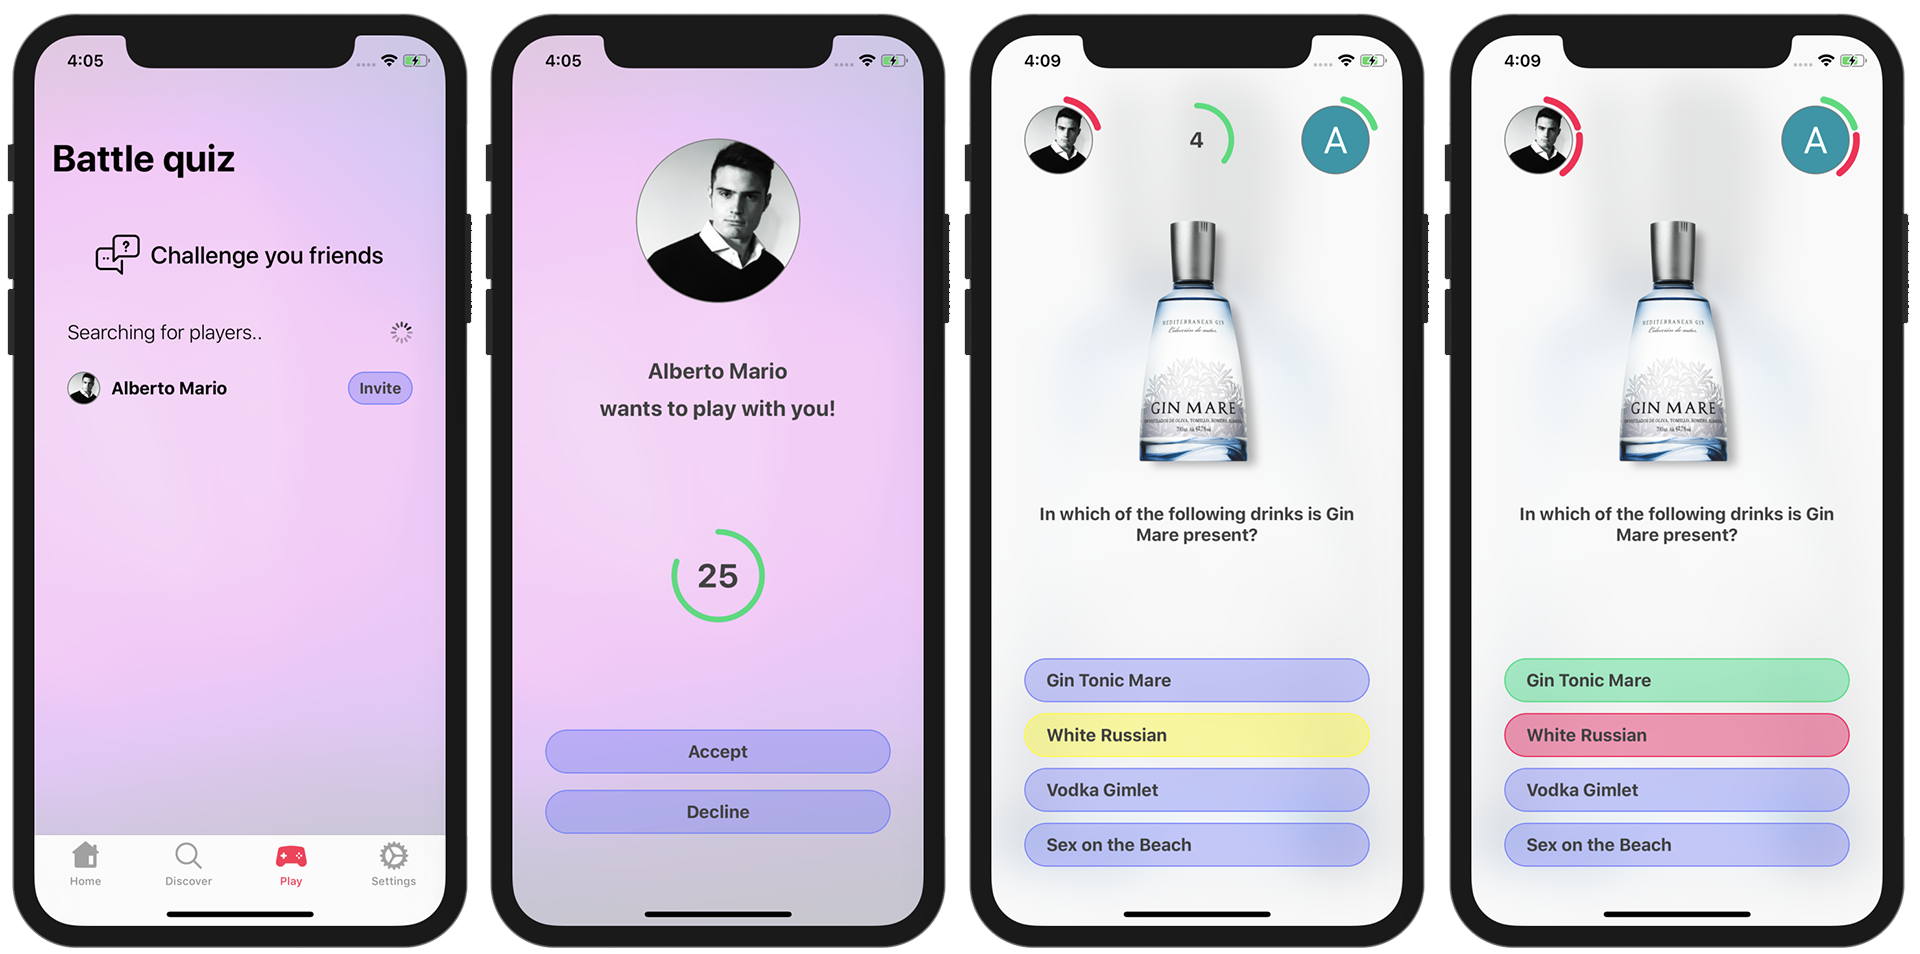
\includegraphics[width=\textwidth]{UI/UI-Play.png}
    \caption{Flow of main events in the play section. From left to right: player discovery, incoming invitation, in-game question with selected answer, in-game question with correct answer}
    \label{Play}
\end{center}
\end{figure}


Each player has 10 seconds to answer, otherwise it will be as if he had picked the wrong answer. 

On the top edges of the screen there are the images of the two players (shown only if they had logged in) and their respective score, updated on a per-question basis.

After the five questions have been answered, both players are shown with the outcome of the match which will result in a \textit{Win, Lost or Tie}.

\subsubsection{Settings section}

\begin{figure}[!ht]
\begin{center}
    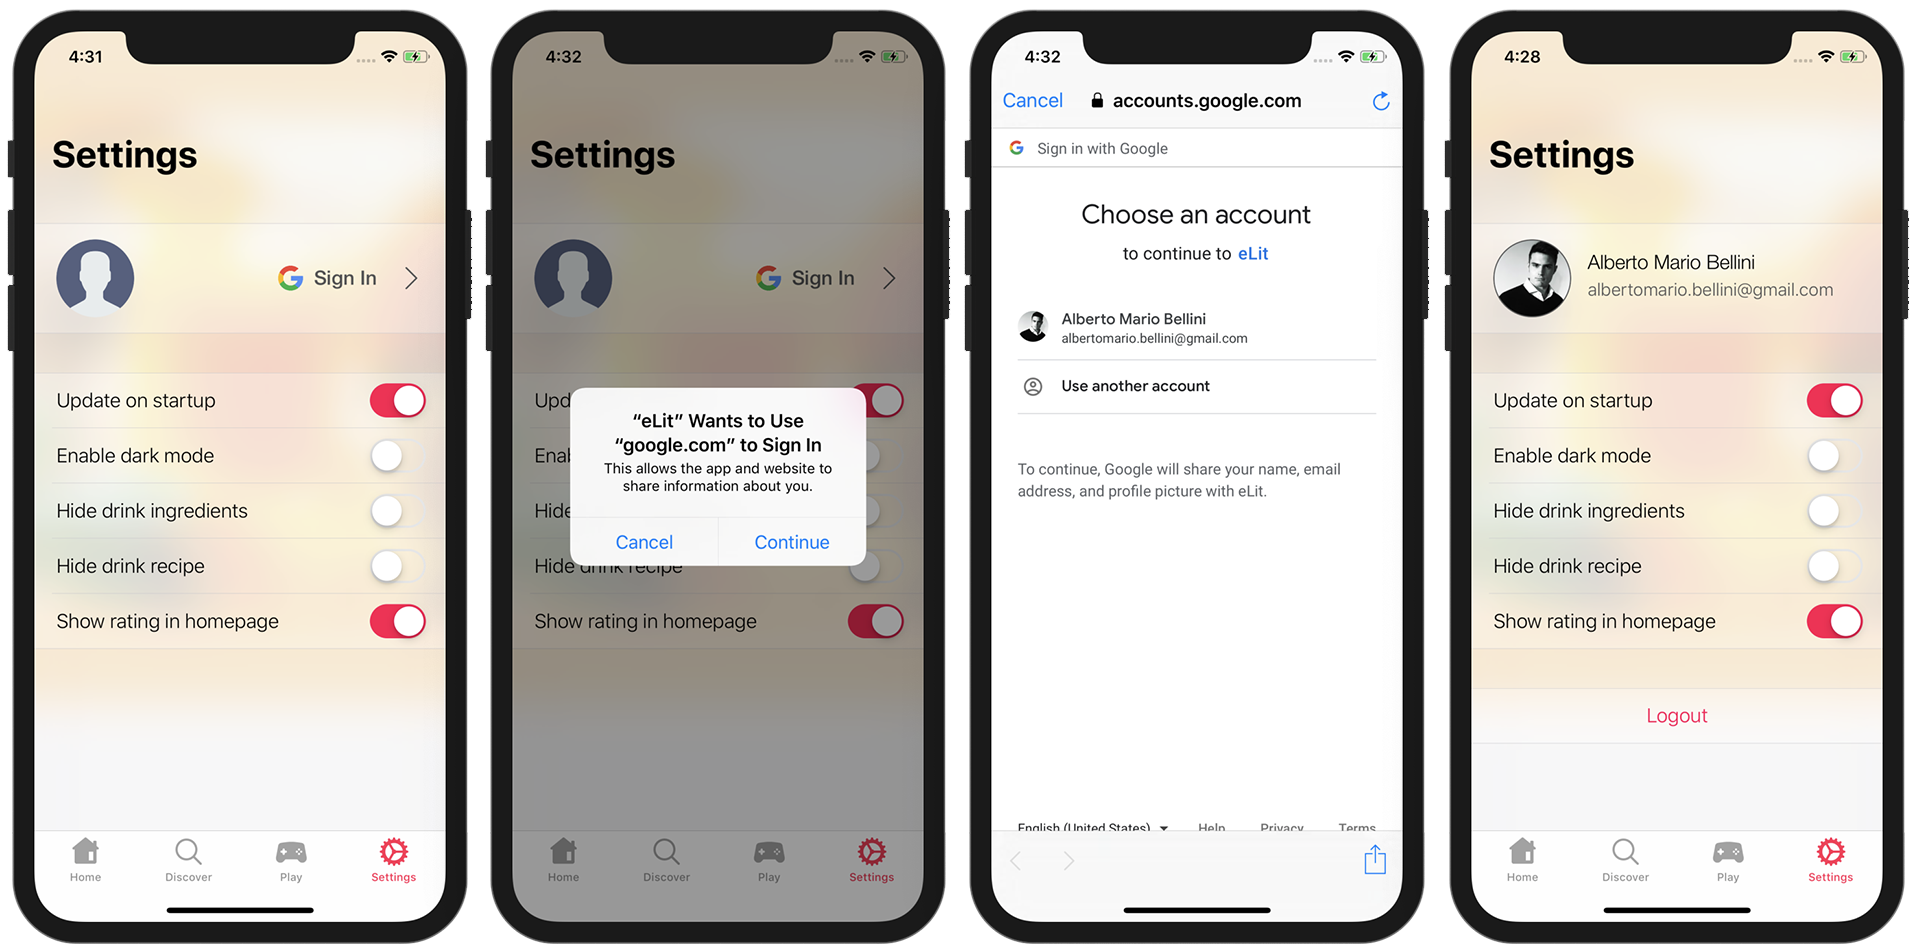
\includegraphics[width=\textwidth]{UI/UI-settings.png}
    \caption{Flow of events in the settings section that allow the user to log-in using his Google account}
    \label{Settings}
\end{center}
\end{figure}

In the last section (see figure \ref{Settings}) we find the settings. Here you can log-in with your Google account and toggle various preference switches, like the one that enables dark mode.

\subsection{Other relevant subsections}

Here we introduce some other relevant UI sections.

\subsubsection{Cocktail detail section}

This section (see figure \ref{Drink detail section}) displays information about a specific cocktail such as title, category, alcoholic degree, description, ingredients, recipe and community reviews. 

To take advantage of the bigger screen of the iPads, the UI has been re-engineered even in this case. Size class tuning wasn't enough to exploit such big screens. For this reason, while on iPhones we have a table-oriented layout with information presented sequentially, on iPads we find a more distributed layout with recipes and ingredients displayed differently.


\begin{figure}
\begin{center}
    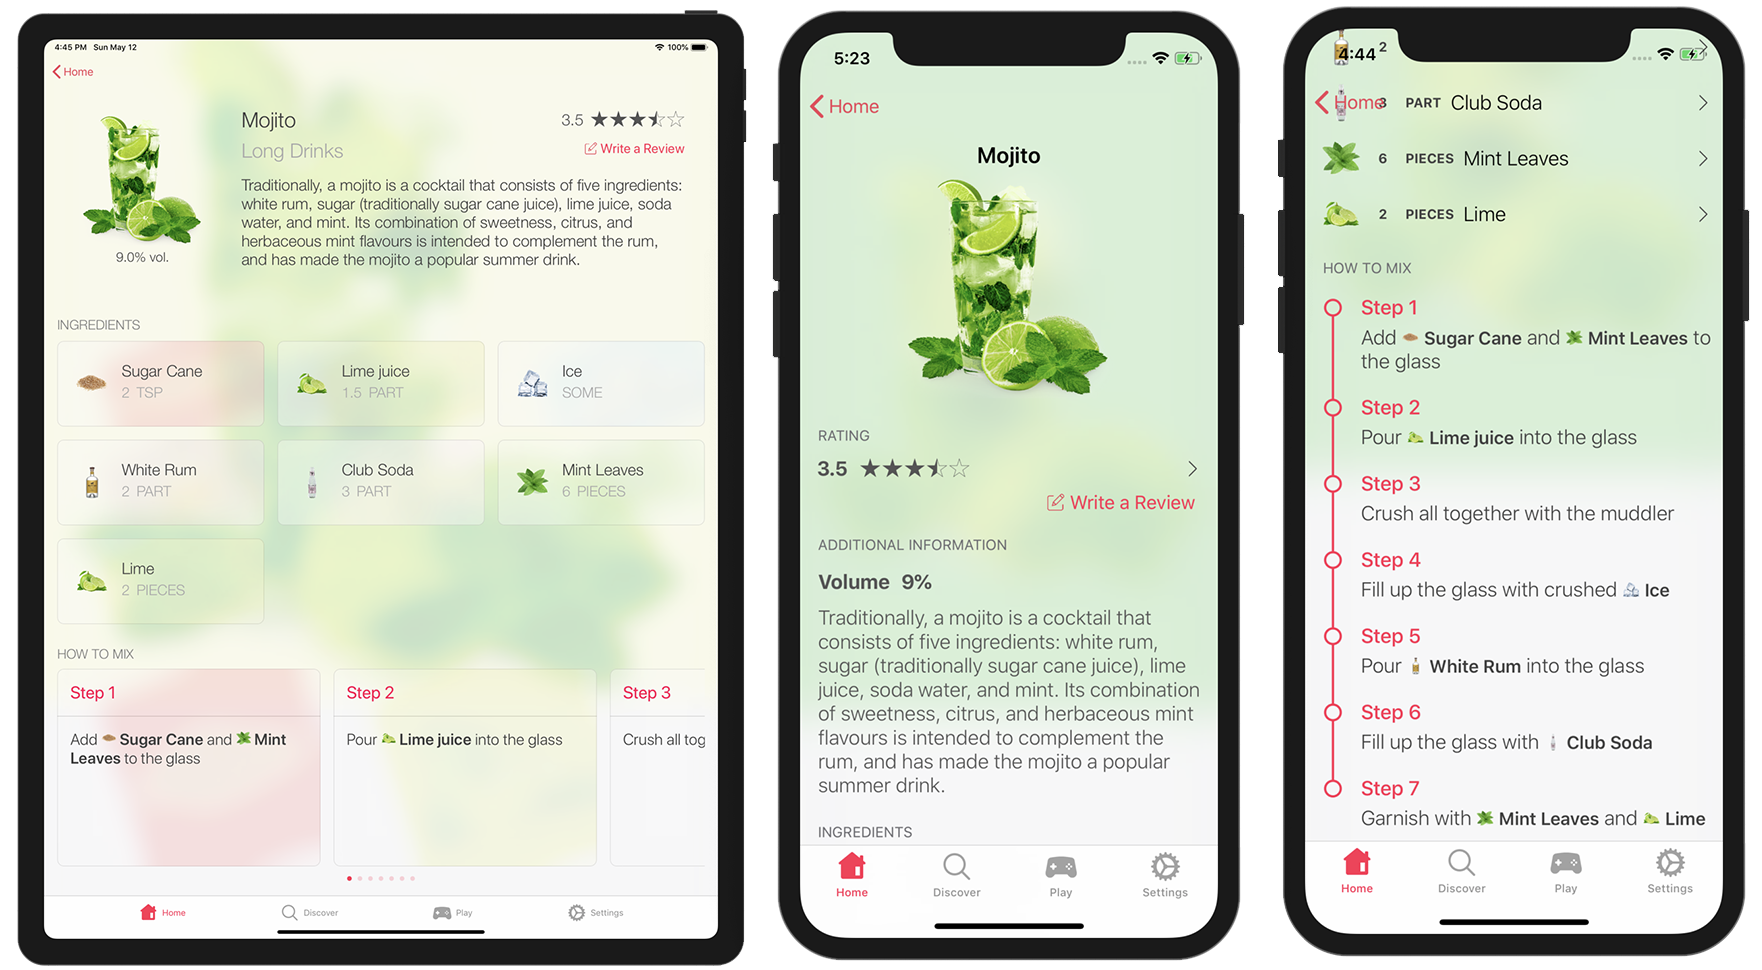
\includegraphics[width=\textwidth]{UI/UI-Drink.png}
    \caption{Different layout of the drink detail section on iPad and iPhone}
    \label{Drink detail section}
\end{center}
\end{figure}

We thought that such change in the layout would have benefit the final user experience on each of the mentioned devices, giving them the feeling of using a robust application designed with accuracy to match the screen size.

The recipe step descriptions make use of ingredients. In order to make it simpler to follow these instruction we opted to add, whenever mentioned, the ingredient image inside the descriptions. The image is the same one displayed in the ingredient section.

Furthermore, touching the rating will show all the reviews for that drink and touching on any ingredient will show all cocktails that can be made with it.

Finally, you can leave your own rating just by tapping on the \textit{Write review} button, assuming you have already logged-in. 

\clearpage
\section{Run time view}
In this section we will show some Run Time views in order to show how the different components interact each other. Some high level components inside the application have been separated in order to better specify the interactions. For the server side we will provide an high level view of the application server; we have also separated it from the db since they are different processes running on the same machine.

\subsection{Rate drink}\label{section : Rate drink}
This Run-time View is showing the steps necessary to write and submit a review for a specific drink.

We start from the assumption that an internet connection is present and that the user is on the cocktail detail page.\\
As shown in figure \ref{Add drink rt} we have four main component that need to interact each other for sending the review to the remote DB:
\begin{itemize}
    \item The \textit{User} is the main component since he has to interact with the application and write the review.
    \item The \textit{Main application} is composed by the user interface and the main controllers attached to it.
    \item The \textit{Network interface} is the component present inside the application that takes the high level requests (in this case the review for a certain drink written by the user) and sends them to the application server through an http POST request.
    \item The \textit{Server} takes care of processing the request coming from the clients and makes the query for insert or update the reviews
    \item The \textit{Database} is the place where reviews are saved so that they can be viewed by all users.
\end{itemize}
We separated the case in which the user has already written a review for the same drink in the past since every user can write only one review per drink. In the case one review is already present in the DB this one is loaded and displayed to the user so that he can edit it.
\begin{figure}[H]
\begin{center}
    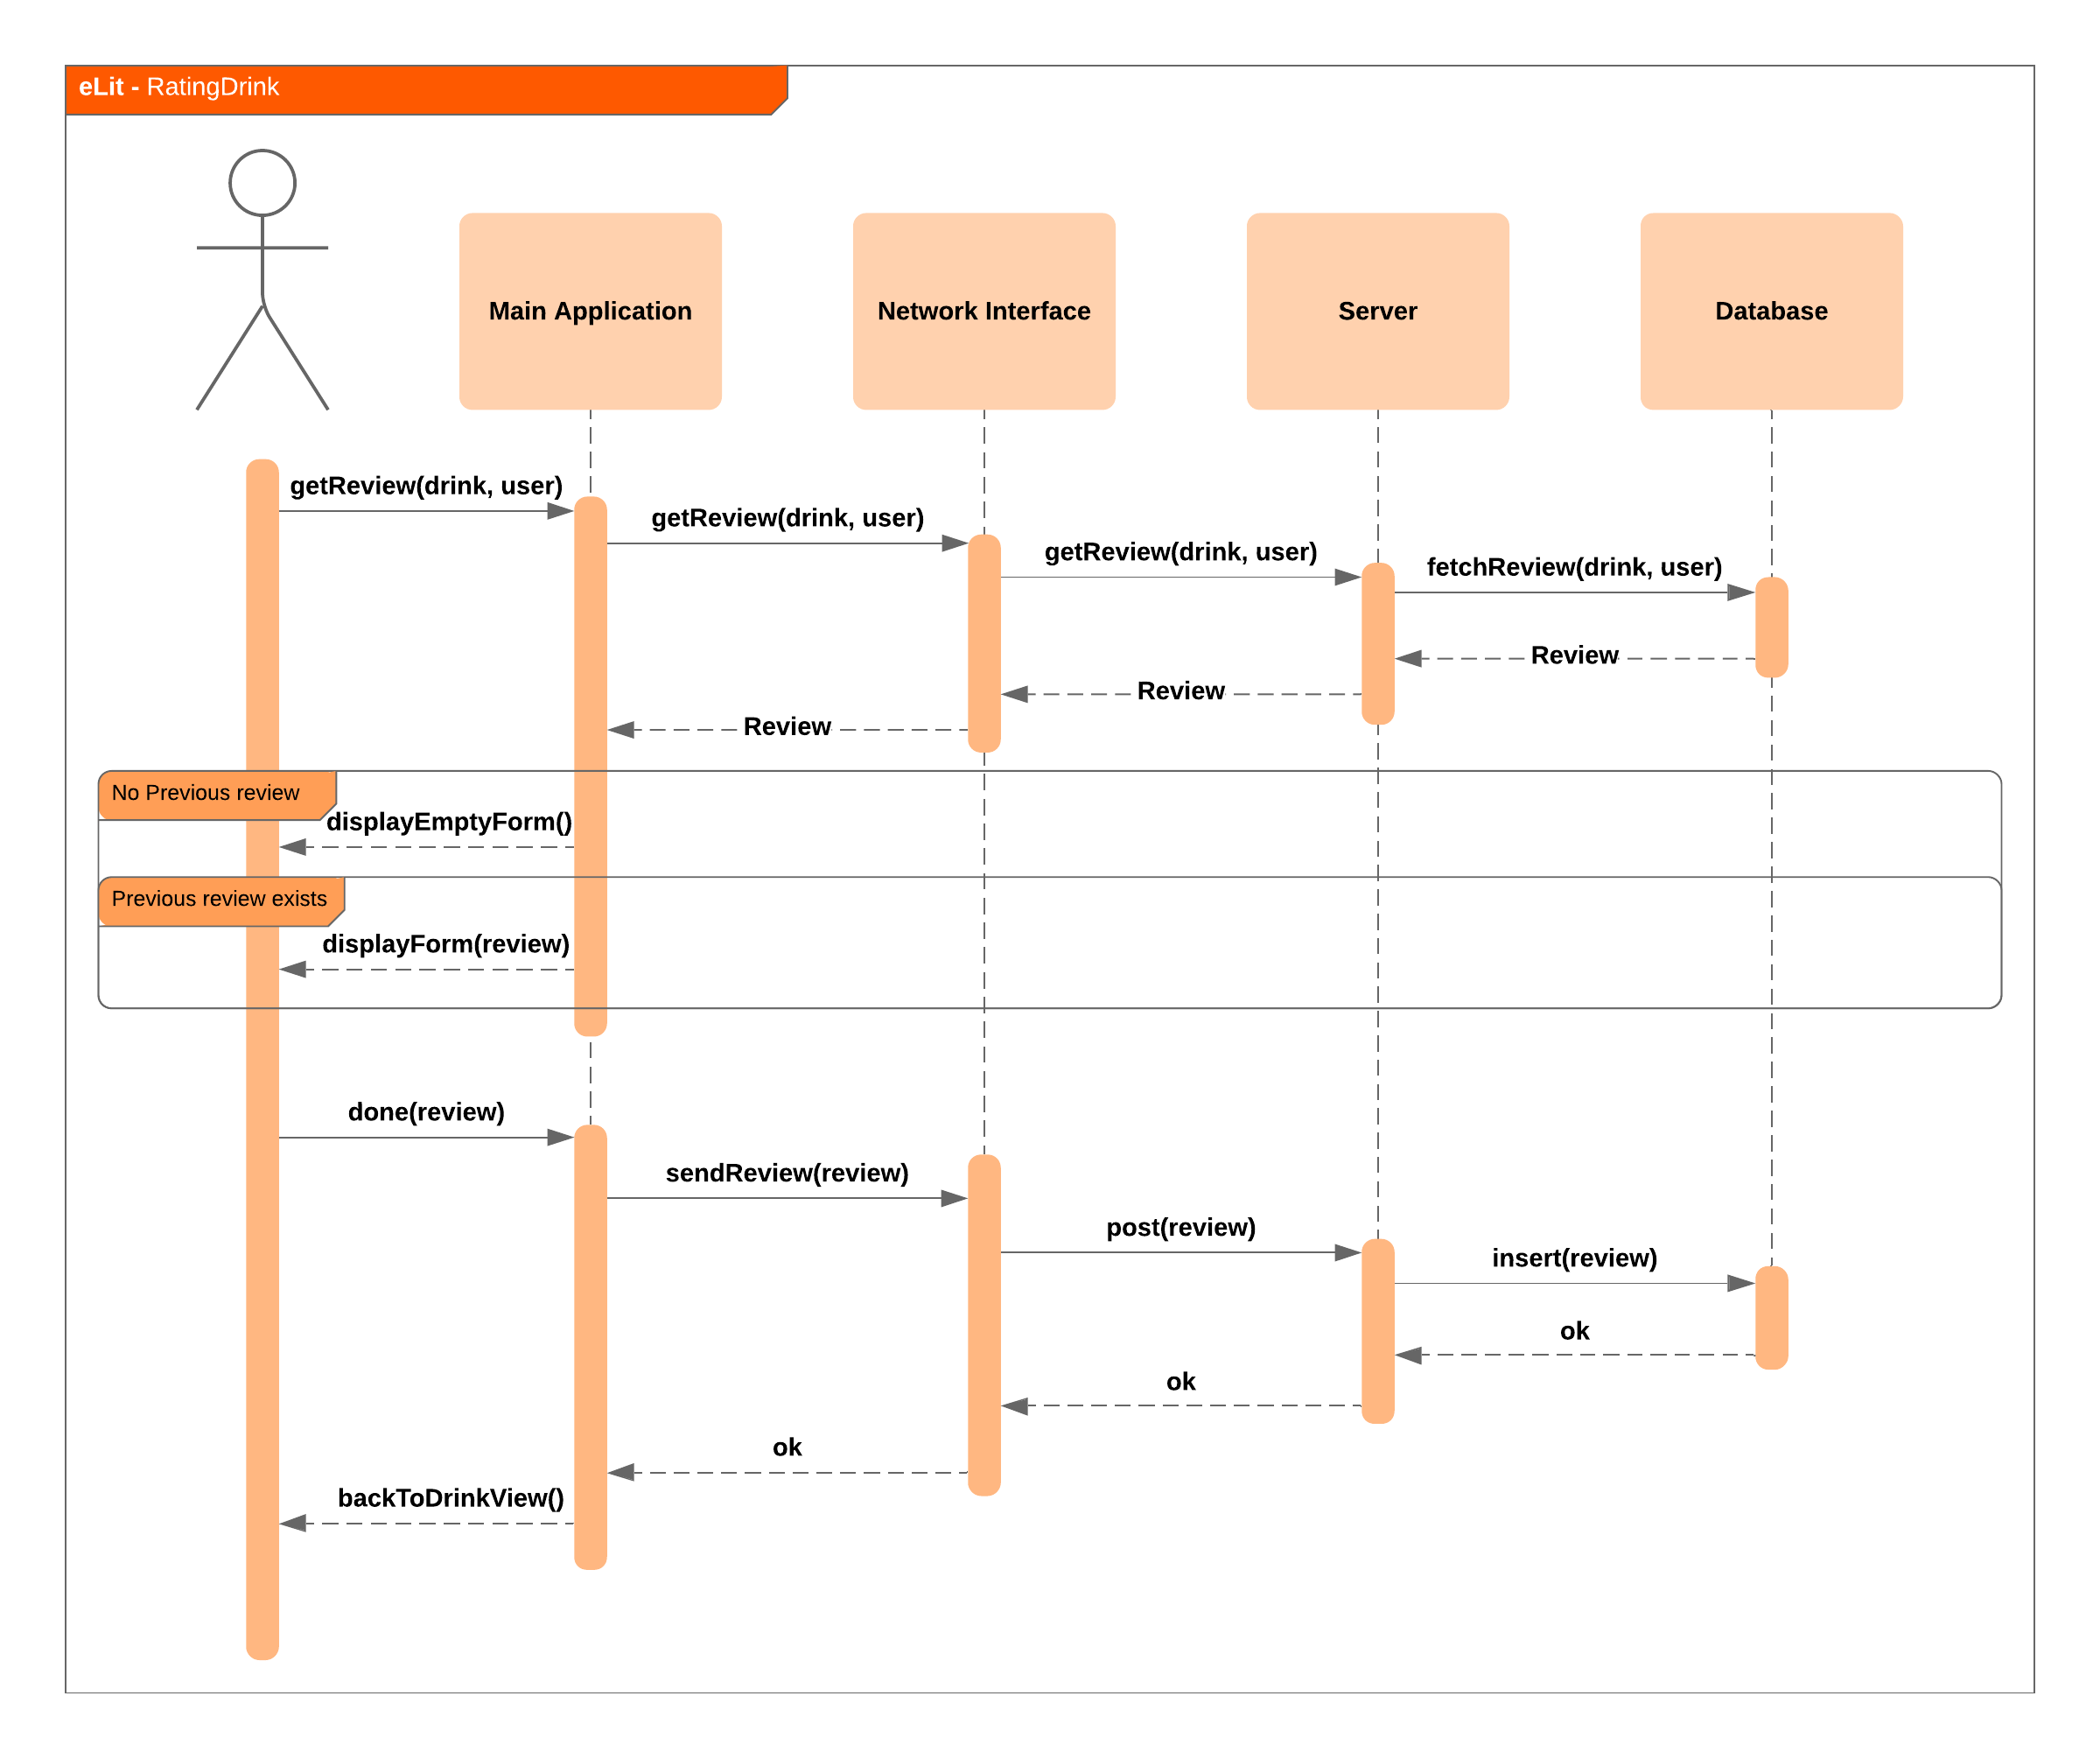
\includegraphics[width=\textwidth]{RunTime/addDrinkReview.png}
    \caption{Add review to drink - Run-time view}
    \label{Add drink rt}
\end{center}
\end{figure}

\newpage
\subsection{Invite friend to play}
This run-time view is showing the steps necessary to invite a friend to play at \textit{Battle Quiz}. We suppose that there are two users with the application installed and running in an iOS device (both iPad or iPhone) and that both of them have the WiFi and Bluetooth enabled (not necessary connected to the Internet.\\
This view refers to the use case 5 presented in section \ref{section:use case}.
As shown in figure \ref{Invite friend rt} we have the following components:
\begin{itemize}
    \item The \textit{User}, as in the previous section (\ref{section : Rate drink}), interacts directly with the application
    \item The \textit{Main application}, as before (section \ref{section : Rate drink}), is composed by the user interface and interacts with the logic layer of the application.
    \item The \textit{Game Engine} is the most important component for the game routine. It is responsible of starting a new game, managing timing, giving questions and answers to the user interface, keeping track of the correct and wrong answers and to determine if the user has won or lost the game. In this view it's only aim is to start the game when the remote client has accepted the invitation.
    \item The \textit{Connection Manager} takes charge of exchanging information with the remote client using the Apple's protocol MultiPeerConnectivity that we have used for discover nearby clients that wants to play and for connect them.
    \item the \textit{Remote Client} is composed by the remote user that we assume being in a certain range from the actual user (in order to be discoverable with our protocol), the main application of the remote user that we assume being in the game tab and so effectively discoverable and the other component of the application on the remote side.
\end{itemize}
In this view we focus only on one side of the two client interacting for starting a game because since the application is the same on both side, also the interfaces and the run-time view is the same. For the remote client, all the components we have presented before for are resumed in the component Remote Client inside figure \ref{Invite friend rt}

\begin{figure}[H]
\begin{center}
    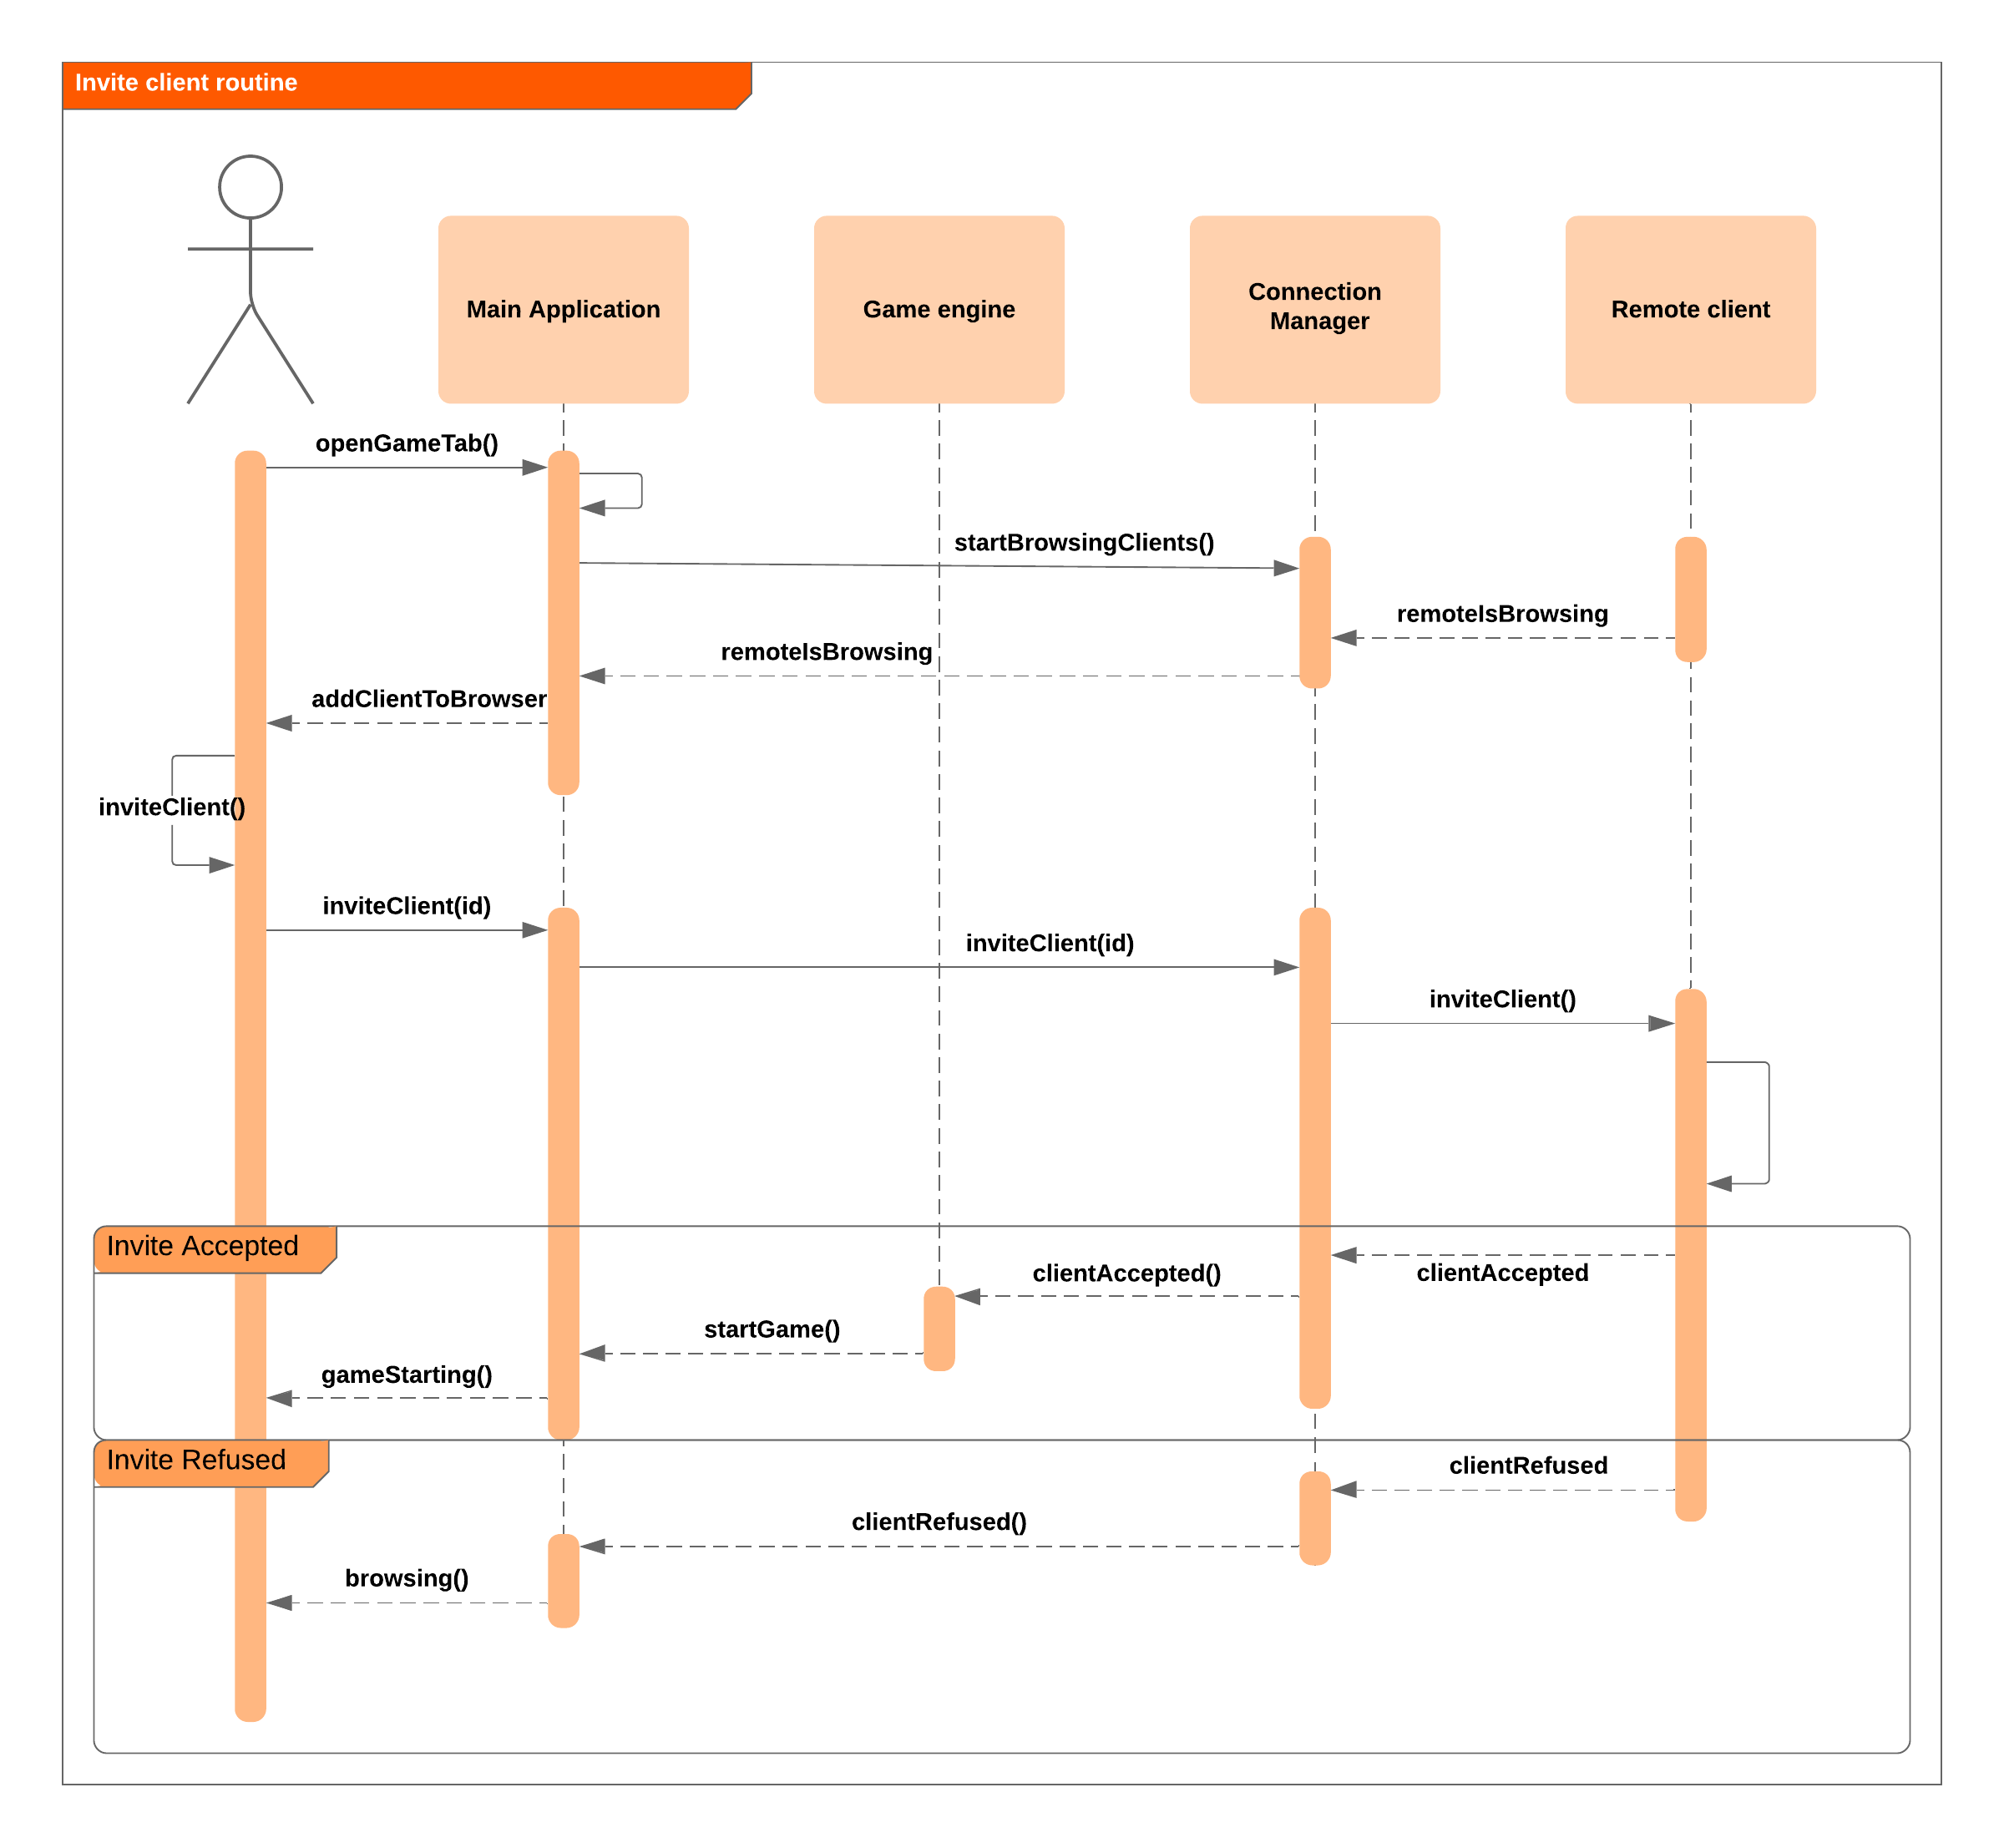
\includegraphics[width=\textwidth]{RunTime/InviteFriend.png}
    \caption{Invite friend to play - Run-time view}
    \label{Invite friend rt}
\end{center}
\end{figure}

\newpage
\subsection{Scan bar-code + drink search}
This run-time view is showing the steps necessary to search all the drinks that can be made with a certain ingredient given his bar-code that can be easily found in most of the bottles.\\
This view refers to the use case 2 presented in section \ref{section:use case}. It is subdivided into two phases:

\begin{enumerate}
    \item \textbf{bar-code search}: We are using two different services (as presented in section \ref{section:overview} and \ref{section:external services}) the first one (\textit{OpenFoodFacts}) is completely free but has a limited amount of bar-code samples. We first send a request to them, if the item is not found we will send a request in cascade to the second one (\textit{UPCItemDB}) that has a limited number of request that we can made but has a bigger Database.
    \item \textbf{local DB search}: After we get the name of the ingredient we make a search query to the application Database looking for ingredients and drinks with the specific ingredient. This step can be done also manually, without the bar-code scan.
\end{enumerate}

As shown in figure \ref{Scan barcode rt} we have the following components:
\begin{itemize}
    \item \textit{User}: See previous run-time view.
    \item \textit{Main Application}: See previous run-time view.
    \item \textit{Network Interface}: This is the component that will interface with the external services crafting an http request with the scanned bar-code. Since we have two different data sources, we first ask to one, if the bar-code is not found we will send a request to the second one. in the figure we are presenting only one request for sake of simplicity.
    \item \textit{Local Database}: This is the database internal to our application from which we fetch the data needed for the search.
\end{itemize}

\begin{figure}[H]
\begin{center}
    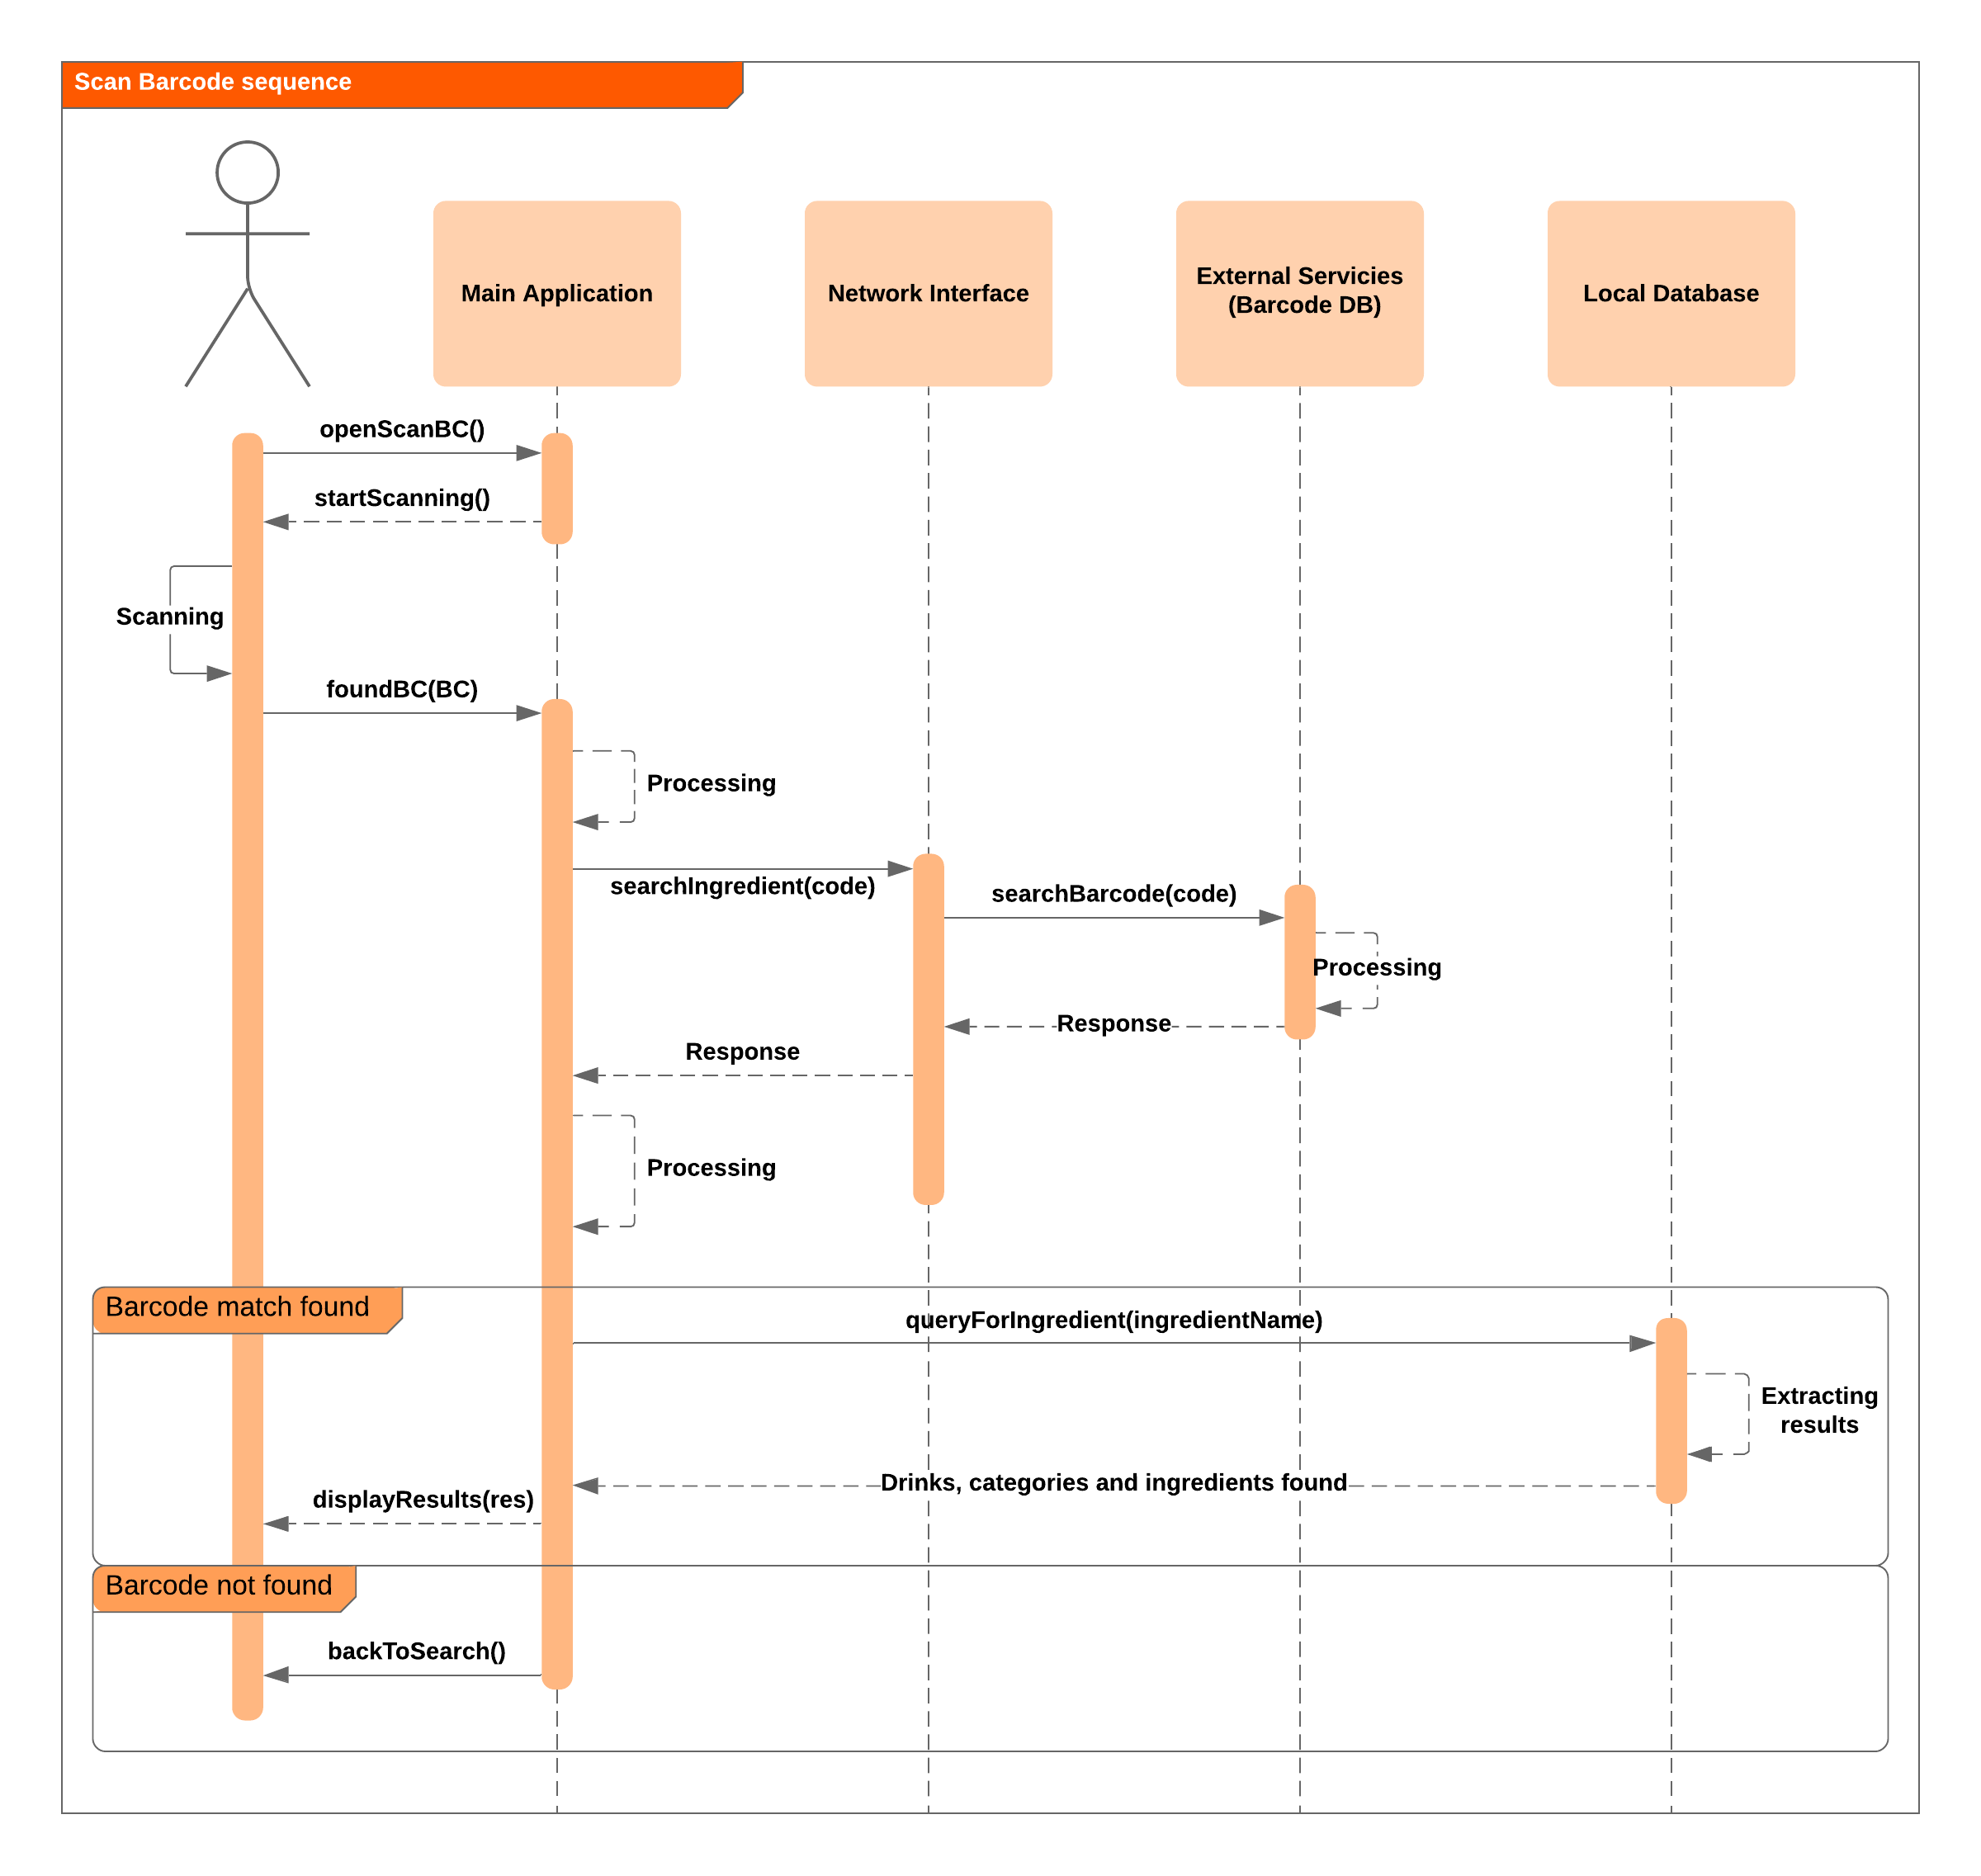
\includegraphics[width=\textwidth]{RunTime/ScanBarcode.png}
    \caption{Scan bar-code and search drinks - Run-time view}
    \label{Scan barcode rt}
\end{center}
\end{figure}

\subsection{Google sign in}

\clearpage
\section{Implementation, integration \& test plan}
In this section we will present the strategies adopted for the design and implementation process. We will describe our working team, the initial design of the application, the steps we have followed for the implementation and some test cases. We will also present the technologies adopted for the application back-end as well as the front-end.

\subsection{Team structure}
Our team is composed by two Computer science engineers with deep knowledge of software engineering and design, networking, algorithm optimization and operating systems.\\
The tasks we'll present have been accomplished by the two members without completely subdivision of tasks among team members.
\begin{itemize}
    \item \textit{Software design}: This task requires strong knowledge of software engineering and design and has been achieved by both members at the start of the implementation process as first step.
    \item \textit{DB design \& back-end implementation}: This task requires strong knowledge of Database design, networking and asynchronous programming. We will present the implementation decisions in section \ref{section: Implementation process}.
    \item \textit{Front-end implementation}: This section requires a good user interface design knowledge and experience and a strong knowledge of software engineering and asynchronous programming for the Controller part of the application.
    \item \textit{Testing}: This task has been made both with UNIT tests and testing by hand some critical parts of the application. We have also made a closed alpha testing with some of our friends.
\end{itemize}

\subsection{Implementation strategy}
\begin{figure}[H]
\begin{center}
    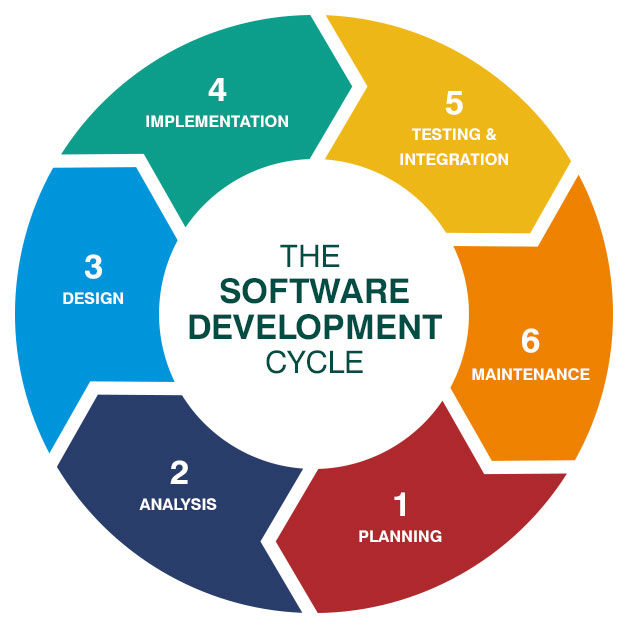
\includegraphics[width=0.4\textwidth]{Implementation.jpg}
    \caption{Software development cycle}
    \label{implementation}
\end{center}
\end{figure}

\subsection{Implementation process}\label{section: Implementation process}
\subsection{Test cases}
\textcolor{red}{
    gian qui mettici roba tipo macchia d'olio o simili, come abbiamo portato avanti il lavoro etc. l'ordine delle cose fatte, come, perchè ? backend ? quando ? python ? perchè ? mongo db ? perchè ? core data ? Perchè ? etc etc. Si possono riempire 2 pagine tranquillamente.  (test esclusi)
}
\end{document}